\chapter[CAPÍTULO IV]{PROPUESTA TÉCNICA DE LA MEJORA}

\section{Plan de Acción de la Mejora Propuesta}

Este capítulo presenta la estrategia de implementación del sistema web help-desk y control de activos TI, formalizada en el \hyperlink{anexo4_acta}{Anexo 4} (\textit{Acta de Constitución del Proyecto}). Para ejecutar la mejora de forma ordenada, el plan se organiza bajo dos enfoques complementarios:

\begin{itemize}
    \item \textbf{Gestión y desarrollo (\textit{Scrumban}):} Combina \textbf{Scrum} para las entregas incrementales por \textit{sprints} y \textbf{Kanban} para el control visual del flujo y límites \textit{WIP} (\textit{Frontend} en Next.js; \textit{Backend} en NestJS con Prisma ORM y MySQL).
    \item \textbf{Analítica y métricas (CRISP-DM):} Estructura el procesamiento del historial de incidencias, activos y auditoría para alimentar los tableros y KPIs gerenciales.
\end{itemize}

A continuación se detallan las metodologías, requerimientos y fases de ejecución del plan.

\subsection{Metodología Scrum}
La metodología \textbf{Scrum} permite gestionar el ciclo de vida del desarrollo del software mediante iteraciones cortas denominadas \textit{sprints}.
\begin{itemize}
\item \textbf{Aplicación en el proyecto:} Se aplica en la planificación y entrega incremental de los módulos del sistema (Módulo de Autenticación y Usuarios, Gestión de Clientes y Sucursales, Gestión de Tickets, Control de Equipos/Hardware o Software, y el motor de Citas).
\item \textbf{Impacto operativo:} Facilita la adaptación continua a los requerimientos prioritarios del negocio mediante la gestión del \textit{Product Backlog} y \textit{Sprint Backlog}, asegurando entregas funcionales probadas al final de cada ciclo de desarrollo.
\end{itemize}

\begin{table}[H]
\centering
\small
\renewcommand{\arraystretch}{1.2}
\caption{Conformación del Equipo Scrum del Proyecto}
\label{tab:equipo_scrum}
\begin{tabular}{@{} p{3.5cm} p{4.5cm} p{6.5cm} @{}}
\toprule
\textbf{Rol Scrum} & \textbf{Integrante} & \textbf{Responsabilidad Principal} \\
\midrule
Product Owner & Julio Flores Vicuña & Define y prioriza los requerimientos del negocio y el \textit{Product Backlog}. \\
Scrum Master / Developer & Jack Daniel Leandro Hernández & Facilita el marco Scrum, remueve impedimentos y participa activamente en la arquitectura y desarrollo de software. \\
Developer & Giovanni Denis Jara Hilario & Participa en el diseño, desarrollo y entregas incrementales del sistema. \\
Developer & Alvaro Jesus Solis Rivadeneyra & Participa en el diseño, desarrollo y entregas incrementales del sistema. \\
\bottomrule
\end{tabular}
\\[0.3em]
{\small \textit{Nota.} Elaboración propia a partir de la organización del equipo de trabajo.}
\end{table}

\subsection{Metodología Kanban}
Implementada para el control visual del flujo operativo de atención de tickets y tareas diarias tanto en la fase de desarrollo como en la operación continua del sistema.
\begin{itemize}
\item \textbf{Aplicación en el proyecto:} En el tablero operativo interactivo donde los analistas de soporte visualizan el ciclo de vida de los tickets (desde que ingresan como \textit{Pendiente}, pasan a \textit{Asignado}, \textit{En Progreso}, \textit{Derivado InSitu}, hasta su \textit{Cierre} o paso a \textit{En Espera Repuesto}).
\item \textbf{Impacto operativo:} Permite limitar el trabajo en curso (\textit{WIP - Work in Progress}), identificar cuellos de botella en tiempo real y transparentar el estado de avance de las atenciones técnicas.
\end{itemize}

\subsection{Metodología CRISP-DM}
Aplicada para estructurar el análisis, procesamiento y minería de los datos generados por la plataforma.
\begin{itemize}
\item \textbf{Aplicación en el proyecto:} En el diseño y estructuración del módulo de \textbf{Dashboard y KPIs}, procesando los datos relacionales de MySQL y los registros en formato JSON de la tabla \texttt{auditoria\_eventos} de la base de datos.
\item \textbf{Impacto operativo:} Garantiza un flujo estructurado en 6 fases (Comprensión del negocio, Comprensión de los datos, Preparación de datos, Modelado, Evaluación y Despliegue) para transformar el historial de incidencias y la carga laboral de los técnicos en métricas de rendimiento precisas para la gerencia.
\end{itemize}

\subsection{Requerimientos del Sistema}
Para el correcto funcionamiento del sistema web help-desk, se han definido y clasificado los requerimientos funcionales y no funcionales que guiarán el desarrollo de la arquitectura y la base de datos.

\subsubsection{Requerimientos Funcionales}
Los requerimientos funcionales especifican las operaciones, interacciones y reglas de negocio que el software debe ejecutar de manera obligatoria para satisfacer las necesidades de los usuarios (administradores, personal técnico y clientes), cuyo detalle operativo se presenta en la Tabla \ref{tab:req_funcionales}.

\begingroup
\footnotesize
\renewcommand{\arraystretch}{1.2}
\begin{longtable}{@{} p{1.8cm} p{3.2cm} p{7.0cm} p{3.2cm} @{}}
\caption{{Requerimientos Funcionales del Sistema}} \label{tab:req_funcionales} \\
\toprule
\textbf{Cod. Req.} & \textbf{Nombre} & \textbf{Descripción} & \textbf{Rol} \\
\midrule
\endfirsthead

\multicolumn{4}{@{}l}{\textbf{Tabla \ref{tab:req_funcionales}} \textit{(Continuación)}} \\[0.4em]
\toprule
\textbf{Cod. Req.} & \textbf{Nombre} & \textbf{Descripción} & \textbf{Rol} \\
\midrule
\endhead

\midrule
\multicolumn{4}{r}{\textit{Continúa en la siguiente página\dots}} \\
\endfoot

\bottomrule
\multicolumn{4}{@{}p{\textwidth}}{\small \textit{Nota.} Detalle completo de los requerimientos funcionales del sistema web help-desk.} \\
\endlastfoot

RF-001 & Gestión de Usuarios y Autenticación & Registro, inicio de sesión con tokens JWT sin estado, cifrado Bcrypt, roles y control de sesiones concurrentes (\textit{soft\_locks}). & ADMIN, SOPORTE, CLIENTE \\
RF-002 & Gestión Organizativa y Planes & Registro y administración de clientes vinculados a un plan de soporte (costo, vigencia y límite de equipos). & ADMINISTRADOR \\
RF-003 & Gestión de Sucursales y Áreas & Administración de sedes físicas y departamentos operativos internos para la ubicación de activos y personal. & ADMIN, CLIENTE \\
RF-004 & Cobertura Geográfica de Técnicos & Asociación mediante tabla pivote (\texttt{tecnicos\_zonas}) de técnicos de campo autorizados por zona geográfica. & ADMINISTRADOR \\
RF-005 & Ciclo de Vida de Tickets & Reporte de incidencias vinculadas a equipos con generación de PIN y gestión de su máquina de estados. & CLIENTE, SOPORTE \\
RF-006 & Parque Informático de Equipos & Registro de equipos de cómputo (Desktop, Laptop) con estado operativo y vinculación al responsable. & ADMIN, SOPORTE \\
RF-007 & Inventario de Hardware & Gestión maestro de componentes físicos, repuestos y su hoja de vida histórica (\texttt{registro\_hardware}). & ADMIN, SOPORTE \\
RF-008 & Gestión de Software y Licencias & Control de catálogo global de software, licencias, claves maestras y acoplamiento por endpoint. & ADMIN, SOPORTE \\
RF-009 & Agendamiento de Visitas In-Situ & Programación de citas de soporte presencial vinculando ticket, técnico, sucursal y control anti-cruces. & SOPORTE \\
RF-010 & Auditoría de Eventos Críticos & Registro histórico detallado de cambios sobre tickets y citas utilizando metadatos estructurados JSON. & ADMINISTRADOR \\
RF-011 & Dashboards e Indicadores & Generación de reportes analíticos de volumen de tickets, tiempos de atención y cumplimiento de SLA. & ADMIN, SOPORTE \\
\end{longtable}
\endgroup

\subsubsection{Requerimientos No Funcionales}
Los requerimientos no funcionales definen los atributos de calidad del sistema, tales como rendimiento, seguridad, disponibilidad, escalabilidad y compatibilidad técnica con los entornos de ejecución, los cuales se consolidan en la Tabla \ref{tab:req_nofuncionales}.

\begingroup
\footnotesize
\renewcommand{\arraystretch}{1.2}
\begin{longtable}{@{} p{1.8cm} p{3.2cm} p{7.0cm} p{3.2cm} @{}}
\caption{{Requerimientos No Funcionales del Sistema}} \label{tab:req_nofuncionales} \\
\toprule
\textbf{Cod. Req.} & \textbf{Nombre} & \textbf{Descripción} & \textbf{Rol} \\
\midrule
\endfirsthead

\multicolumn{4}{@{}l}{\textbf{Tabla \ref{tab:req_nofuncionales}} \textit{(Continuación)}} \\[0.4em]
\toprule
\textbf{Cod. Req.} & \textbf{Nombre} & \textbf{Descripción} & \textbf{Rol} \\
\midrule
\endhead

\midrule
\multicolumn{4}{r}{\textit{Continúa en la siguiente página\dots}} \\
\endfoot

\bottomrule
\multicolumn{4}{@{}p{\textwidth}}{\small \textit{Nota.} Especificaciones de calidad y rendimiento técnico del sistema.} \\
\endlastfoot

RNF-001 & Comunicación en Tiempo Real & Transmisión bidireccional y de baja latencia para notificaciones y estados de tickets mediante WebSockets. & Todos los roles \\
RNF-002 & Seguridad e Integridad & Autenticación segura mediante JWT sin estado, Bcrypt y control de acceso basado en roles (RBAC). & Todos los roles \\
RNF-003 & Persistencia y Escalabilidad & Uso de base de datos relacional MySQL con Prisma ORM y soporte para metadatos JSON dinámicos. & ADMIN, SOPORTE \\
RNF-004 & Rendimiento en Búsquedas & Procesamiento de consultas masivas de inventario y reportes de dashboard en menos de 3 segundos. & ADMIN, SOPORTE \\
RNF-005 & Disponibilidad y Concurrencia & Garantizar 99.8\% de disponibilidad para acceso simultáneo apoyado en bloqueos temporales (\textit{soft\_locks}). & Todos los roles \\
RNF-006 & Arquitectura Limpia & Backend estructurado en NestJS bajo Arquitectura Hexagonal y principios SOLID para alta mantenibilidad. & ADMIN, SOPORTE \\
RNF-007 & Trazabilidad y Auditoría & Registro automatizado de eventos críticos e historiales en tablas de auditoría y hojas de vida. & ADMIN, SOPORTE \\
RNF-008 & Compatibilidad Responsive & Interfaz frontend adaptable a distintos dispositivos y navegadores web modernos (Chrome, Edge, Firefox). & Todos los roles \\
\end{longtable}
\endgroup

\subsection{Fases del Plan de Acción por Sprints}
El desarrollo e implementación de la mejora en J\&P Periféricos S.A.C. se estructura cronológicamente en iteraciones cortas agrupadas en fases técnicas, permitiendo asegurar entregas incrementales y controladas de la solución.

\subsubsection{Fase 1: Análisis y Modelado (Sprints 0 - 1)}
Esta fase inicial comprende la recopilación de especificaciones, el diseño conceptual de la arquitectura de datos, el modelado de procesos y la definición formal de los diagramas UML, cuyas actividades y plazos se detallan en la Tabla \ref{tab:fase1}.

\begingroup
\small
\renewcommand{\arraystretch}{1.25}
\begin{longtable}{@{} p{3.2cm} p{8.8cm} p{3.0cm} @{}}
\caption{{Fase 1: Análisis y Modelado (Sprints 0 - 1)}} \label{tab:fase1} \\
\toprule
\textbf{Actividad / Tarea} & \textbf{Descripción del Entregable} & \textbf{Duración / Plazo} \\
\midrule
\endfirsthead

\multicolumn{3}{@{}l}{\textbf{Tabla \ref{tab:fase1}} \textit{(Continuación)}} \\[0.4em]
\toprule
\textbf{Actividad / Tarea} & \textbf{Descripción del Entregable} & \textbf{Duración / Plazo} \\
\midrule
\endhead

\midrule
\multicolumn{3}{r}{\textit{Continúa en la siguiente página\dots}} \\
\endfoot

\bottomrule
\multicolumn{3}{@{}p{\textwidth}}{\small \textit{Nota.} Cronograma y entregables detallados para la fase de análisis y modelado.} \\
\endlastfoot

TR00 - Planificación y gestión del proyecto & Planificación, ceremonias de sprint, revisiones y documentación transversal. & 14 días \\
TR01 - Alcance y Problemática & Definición del alcance del proyecto y problemática de trazabilidad TI. & 4 días \\
TR02 - Modelado de Negocio & Modelado del flujo de negocio y matriz de permisos por rol. & 5 días \\
TR03 - Requisitos & Redacción de especificación de Requisitos Funcionales y No Funcionales. & 5 días \\
TR04 - EDT / WBS & Construcción de la Estructura Desglosada de Trabajo y línea base. & 4 días \\
TR05 - Análisis Hoja de Vida & Análisis de requerimientos para el módulo de Hoja de Vida de Equipos. & 4 días \\
TR06 - Matriz CRUD & Elaboración de matriz CRUD de accesos y permisos por rol. & 4 días \\
TR07 - Diagramas UML & Diseño de diagramas UML y especificaciones de Casos de Uso. & 6 días \\
TR08 - Esquema Relacional & Creación del esquema relacional y enums en \texttt{schema.prisma}. & 4 días \\
\textbf{Total Fase 1} & & \textbf{50 días} \\
\end{longtable}
\endgroup

Como evidencia del cumplimiento de esta fase inicial, a continuación se presentan los tableros de gestión, los gráficos de seguimiento (\textit{burndown charts}) y el diseño del esquema de base de datos (tarea TR08):

\begin{figure}[H]
\centering
\captionsetup{justification=centering}
\caption{Tablero de Jira - Sprint 0 }
\label{fig:evidencia_sprint_0}
\vspace{0.2em}
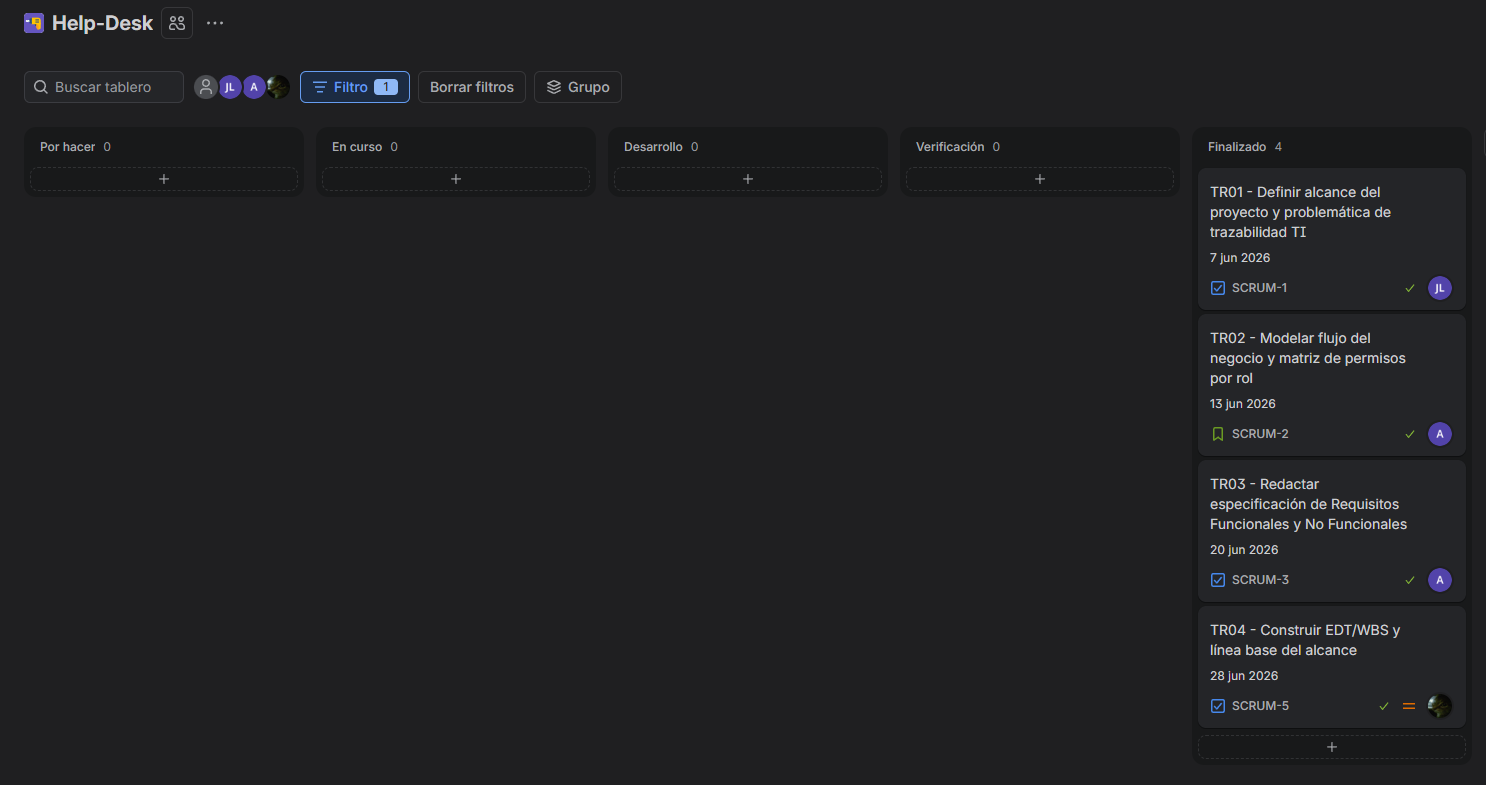
\includegraphics[width=0.92\textwidth]{tablero_sprint_0.png}
\\[0.2em]
{\small \textit{Nota.} Vista general del tablero de tareas correspondiente al análisis, modelado de negocio y arquitectura base}
\end{figure}

\begin{figure}[H]
\centering
\captionsetup{justification=centering}
\caption{Burndown Chart - Sprint 0}
\label{fig:burndown_sprint_0}
\vspace{0.2em}
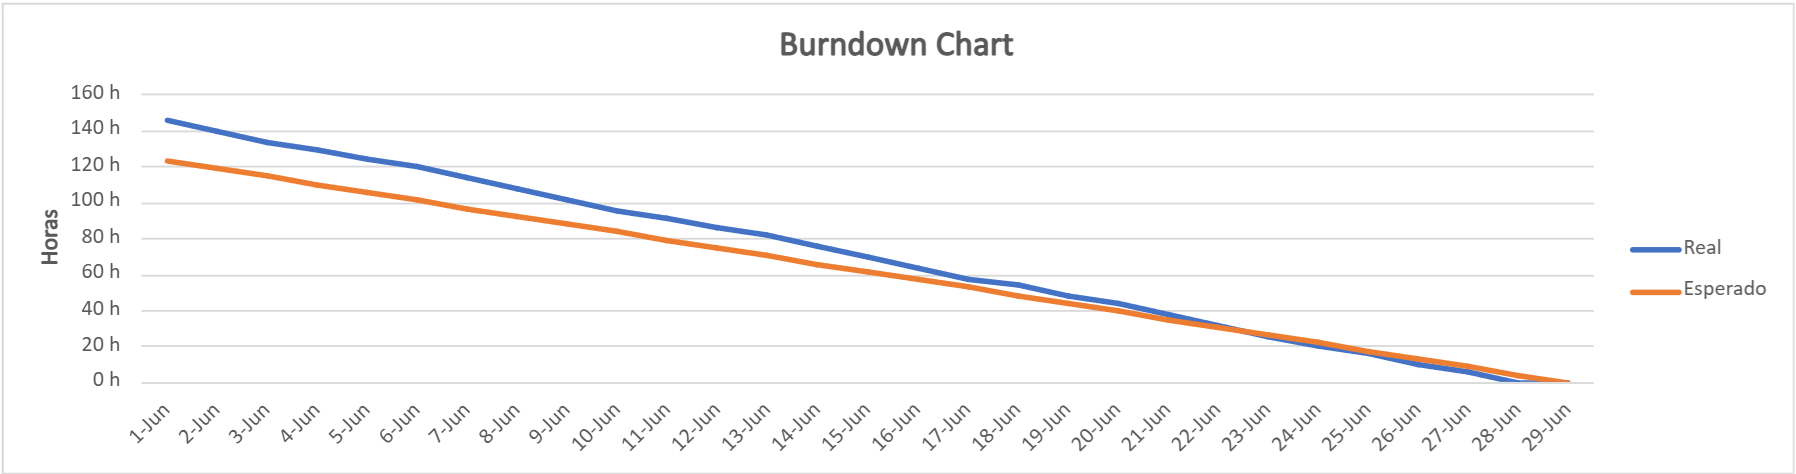
\includegraphics[width=0.92\textwidth]{burdowchart_sprint0.png}
\\[0.2em]
{\small \textit{Nota.} Elaboración propia. Seguimiento de horas estimadas frente al avance real durante el Sprint 0.}
\end{figure}

\begin{figure}[H]
\centering
\captionsetup{justification=centering}
\caption{Tablero de Jira - Sprint 1}
\label{fig:evidencia_sprint_1}
\vspace{0.2em}
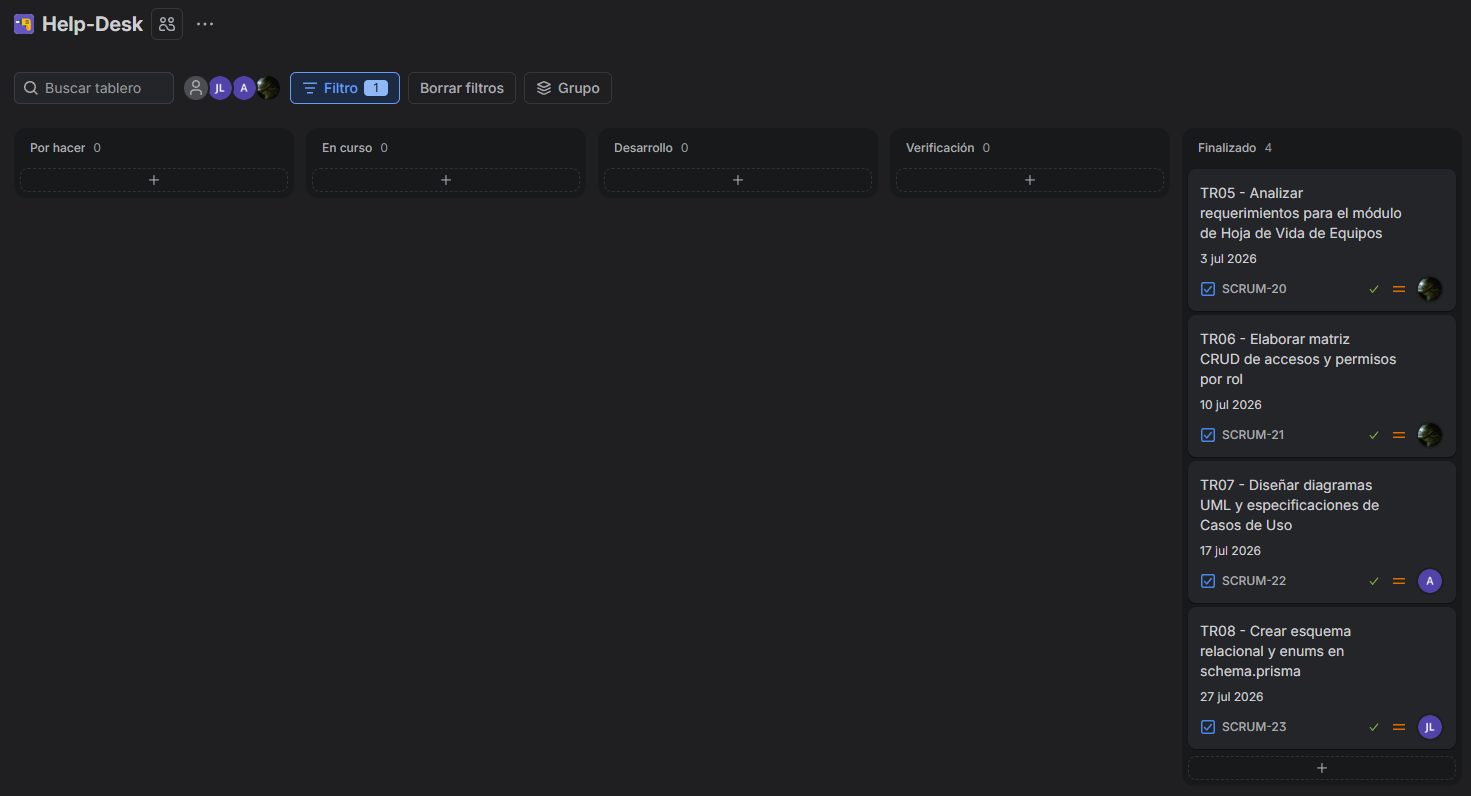
\includegraphics[width=0.92\textwidth]{tablero_sprint_1.png}
\\[0.2em]
{\small \textit{Nota.} Vista general del tablero de tareas correspondiente al análisis detallado, diagramas UML y configuración inicial Backend}
\end{figure}

\begin{figure}[H]
\centering
\captionsetup{justification=centering}
\caption{Burndown Chart - Sprint 1}
\label{fig:burndown_sprint_1}
\vspace{0.2em}
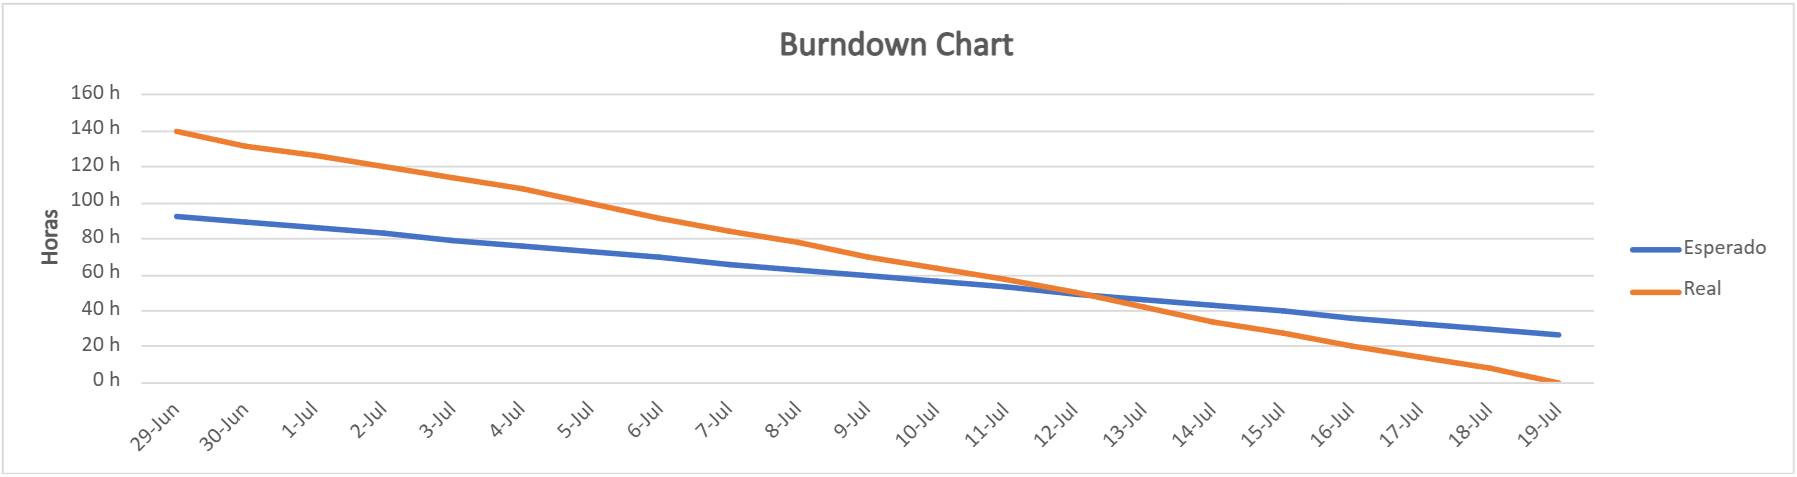
\includegraphics[width=0.92\textwidth]{burdowchart_sprint1.png}
\\[0.2em]
{\small \textit{Nota.} Elaboración propia. Seguimiento de horas estimadas frente al avance real durante el Sprint 1.}
\end{figure}

\begin{figure}[H]
\centering
\captionsetup{justification=centering}
\caption{Esquema Relacional implementado en \texttt{schema.prisma}}
\label{fig:evidencia_schema_prisma}
\vspace{0.2em}
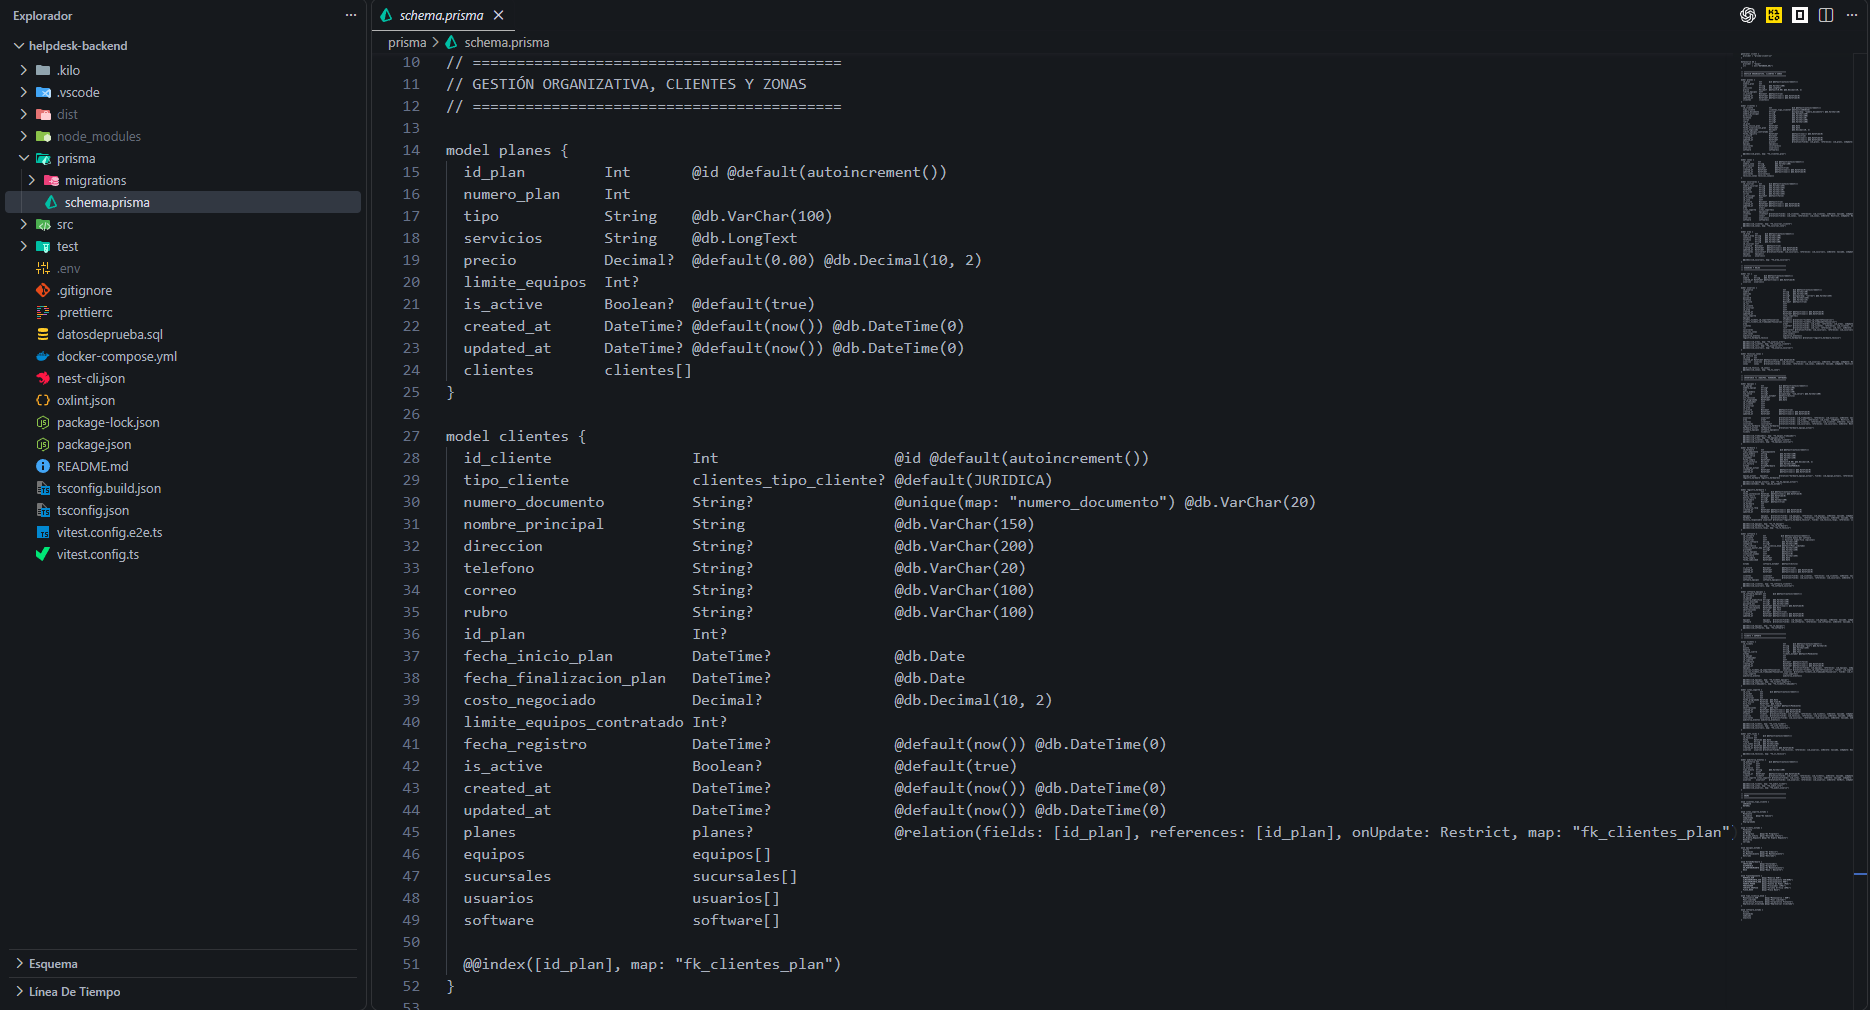
\includegraphics[width=0.92\textwidth]{schema_prisma.png}
\\[0.2em]
{\small \textit{Nota.} Definición de modelos, entidades y enumeraciones relacionales en el archivo de configuración de Prisma.}
\end{figure}

\subsubsection{Fase 2: Backend Core y Módulos Iniciales (Sprints 2 - 3)}
Durante esta etapa se ejecuta la construcción principal de la lógica del servidor, implementando los módulos de autenticación segura, gestión de usuarios, clientes, sucursales, planes SLA y el control transaccional del inventario ITAM, cuyas tareas ejecutadas se presentan en la Tabla \ref{tab:fase2}.

\begingroup
\small
\renewcommand{\arraystretch}{1.25}
\begin{longtable}{@{} p{3.2cm} p{8.8cm} p{3.0cm} @{}}
\caption{{Fase 2: Backend Core y Módulos Iniciales (Sprints 2 - 3)}} \label{tab:fase2} \\
\toprule
\textbf{Actividad / Tarea} & \textbf{Descripción del Entregable} & \textbf{Duración / Plazo} \\
\midrule
\endfirsthead

\multicolumn{3}{@{}l}{\textbf{Tabla \ref{tab:fase2}} \textit{(Continuación)}} \\[0.4em]
\toprule
\textbf{Actividad / Tarea} & \textbf{Descripción del Entregable} & \textbf{Duración / Plazo} \\
\midrule
\endhead

\midrule
\multicolumn{3}{r}{\textit{Continúa en la siguiente página\dots}} \\
\endfoot

\bottomrule
\multicolumn{3}{@{}p{\textwidth}}{\small \textit{Nota.} Cronograma y entregables detallados para el desarrollo del núcleo del backend.} \\
\endlastfoot

TR09 - Configuración NestJS & Configuración con Arquitectura Hexagonal, Prisma Client y módulo Common. & 5 días \\
TR10 - Autenticación JWT & Desarrollo de Autenticación JWT y Guards de Control de Acceso por Roles. & 5 días \\
TR11 - CRUD Usuarios y Zonas & Implementación de CRUD de Usuarios, Zonas geográficas y Auditoría. & 6 días \\
TR12 - Backend Clientes & Desarrollo del backend de Clientes con flujo de confirmación por correo. & 5 días \\
TR13 - Sucursales y Áreas & Gestión de Sucursales/Áreas y provisión de usuario por sucursal. & 5 días \\
TR14 - Gestión SLA & Implementación de gestión backend de Planes y Acuerdos de Nivel de Servicio. & 5 días \\
TR15 - Lógica Inventario ITAM & Desarrollo de lógica backend de Inventario ITAM y Hoja de Vida de Activos. & 6 días \\
TR16 - Control de Software & Implementación de gestión backend de Software y Control de Licencias. & 5 días \\
TR17 - Ciclo de Vida Ticket & Desarrollo del ciclo de vida del Ticket (estado pendiente y asignación). & 6 días \\
\textbf{Total Fase 2} & & \textbf{48 días} \\
\end{longtable}
\endgroup

Como evidencia de la ejecución del núcleo del servidor y gestión de inventario, se muestran los tableros, los gráficos de seguimiento y la implementación técnica:

\begin{figure}[H]
\centering
\captionsetup{justification=centering}
\caption{Tablero de Jira - Sprint 2}
\label{fig:evidencia_sprint_2}
\vspace{0.2em}
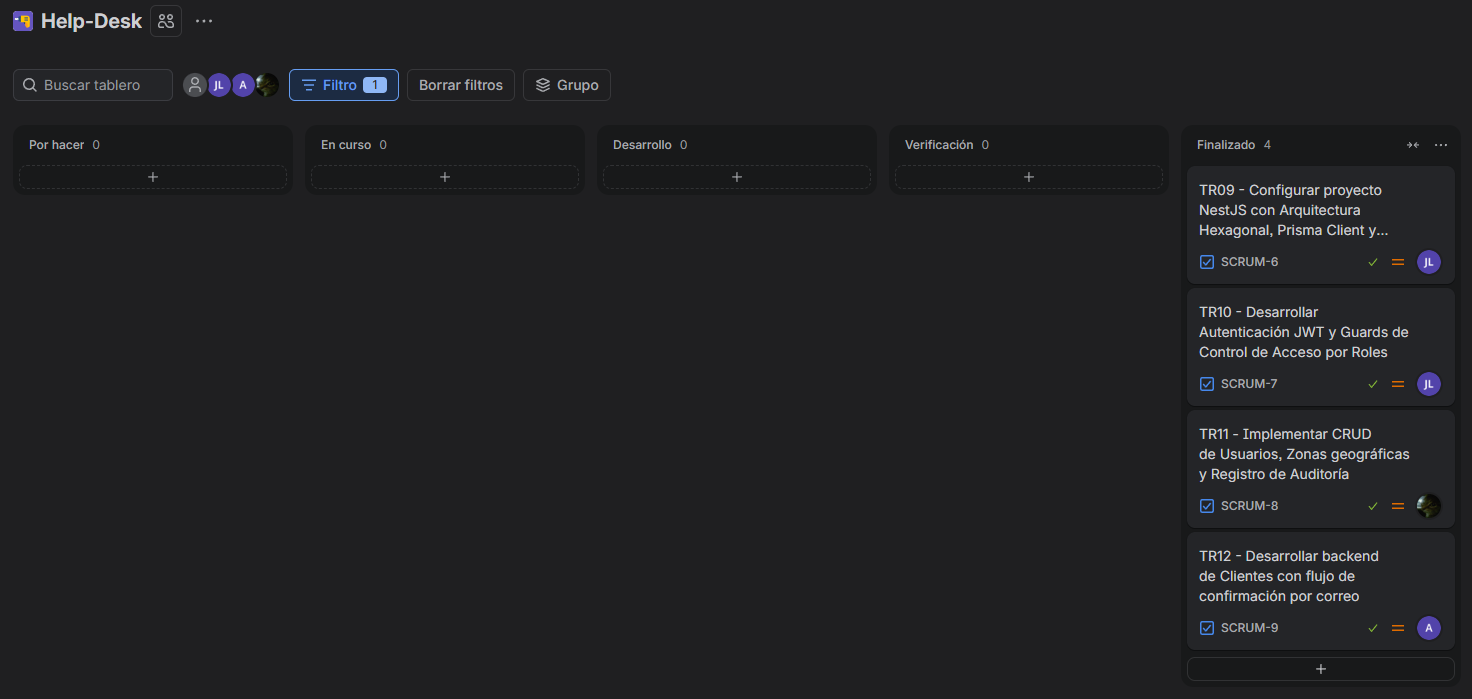
\includegraphics[width=0.92\textwidth]{tablero_sprint_2.png}
\\[0.2em]
{\small \textit{Nota.} Estado de avance del Backend en Autenticación, Usuarios y Jerarquía Organizacional.}
\end{figure}

\begin{figure}[H]
\centering
\captionsetup{justification=centering}
\caption{Burndown Chart - Sprint 2}
\label{fig:burndown_sprint_2}
\vspace{0.2em}
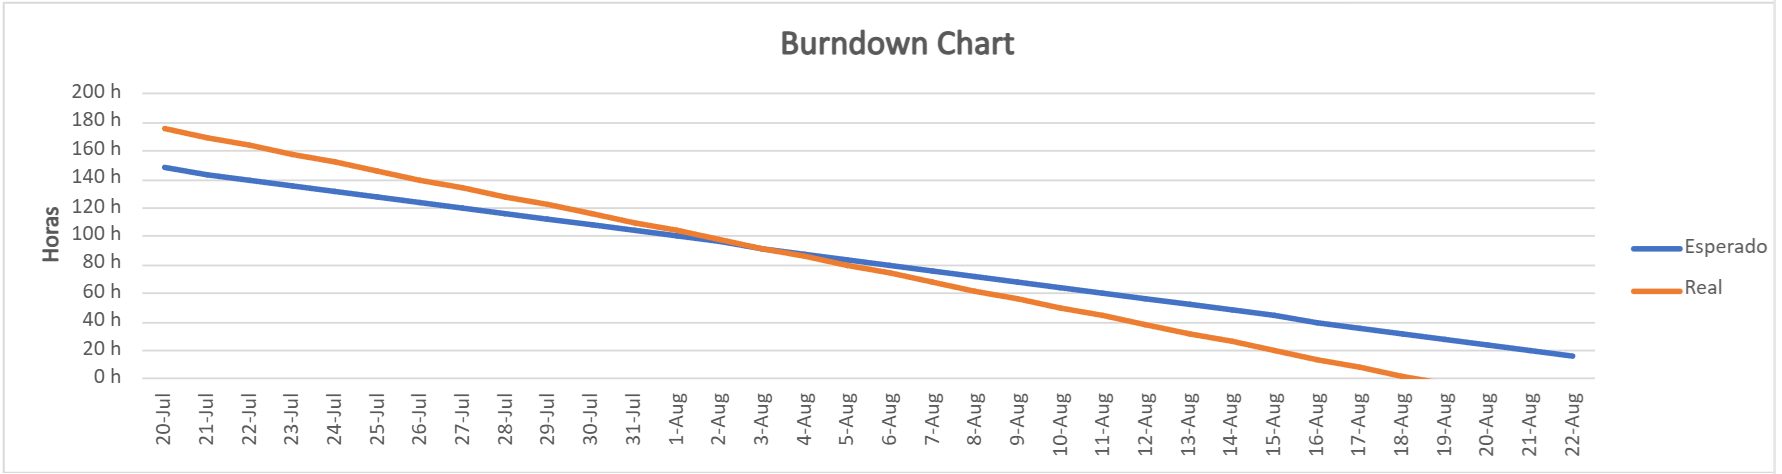
\includegraphics[width=0.92\textwidth]{burdowchart_sprint2.png}
\\[0.2em]
{\small \textit{Nota.} Elaboración propia. Seguimiento de horas estimadas frente al avance real durante el Sprint 2.}
\end{figure}

\begin{figure}[H]
\centering
\captionsetup{justification=centering}
\caption{Tablero de Jira - Sprint 3}
\label{fig:evidencia_sprint_3}
\vspace{0.2em}
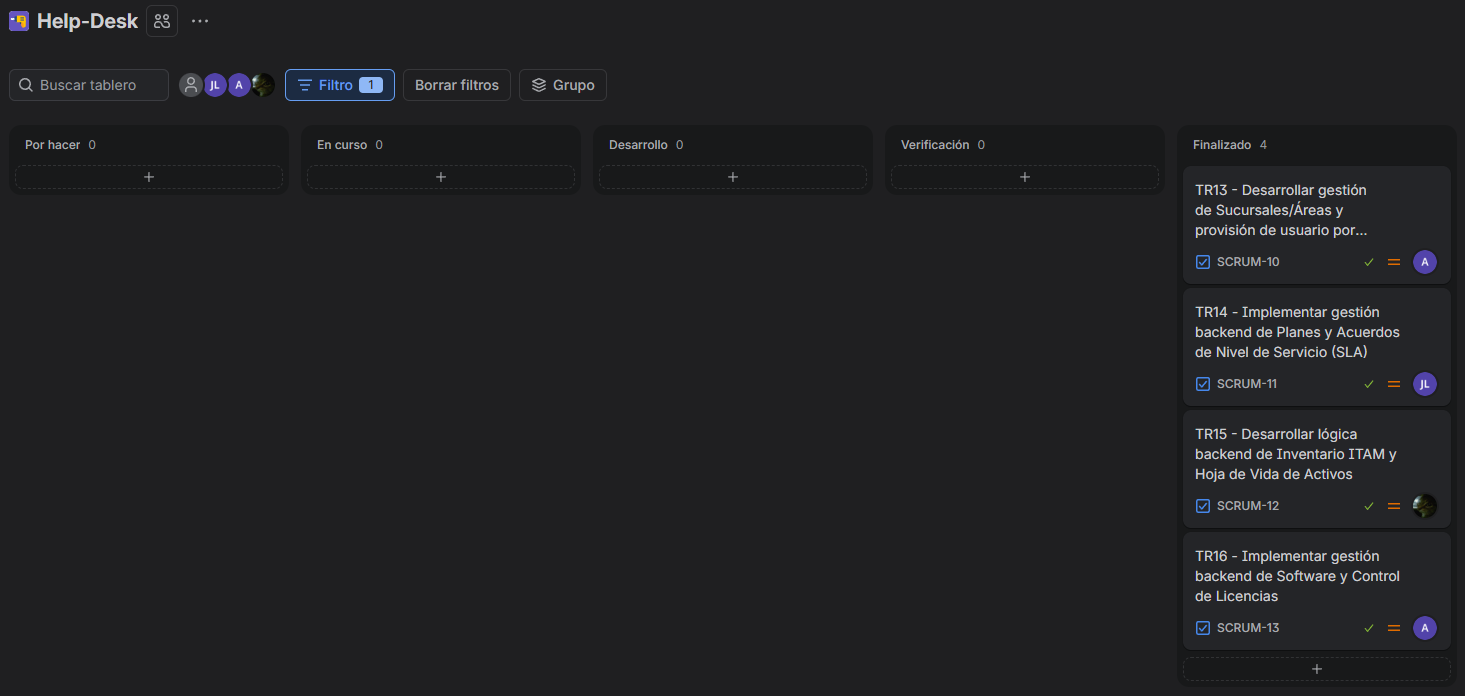
\includegraphics[width=0.92\textwidth]{img/tablero_sprint_3.png}
\\[0.2em]
{\small \textit{Nota.} Estado de avance del Backend en Sucursales, SLA, Inventario ITAM y Licencias.}
\end{figure}

\begin{figure}[H]
\centering
\captionsetup{justification=centering}
\caption{Burndown Chart - Sprint 3}
\label{fig:burndown_sprint_3}
\vspace{0.2em}
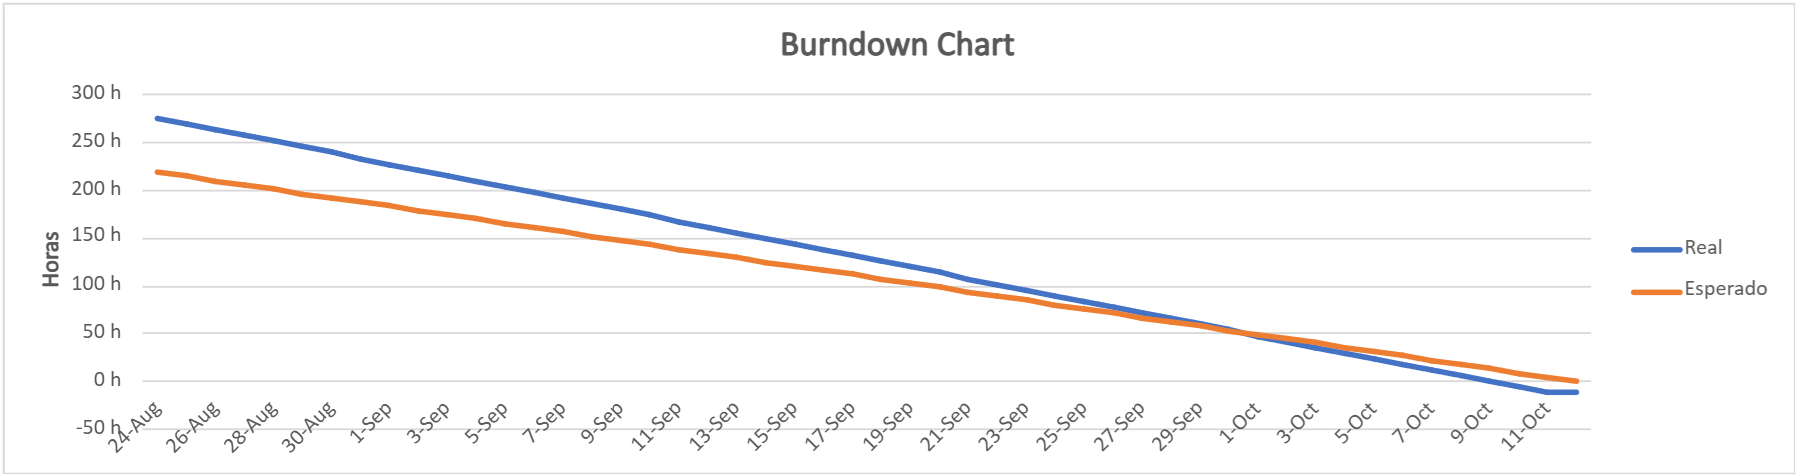
\includegraphics[width=0.92\textwidth]{burdowchart_sprint3.png}
\\[0.2em]
{\small \textit{Nota.} Elaboración propia. Seguimiento de horas estimadas frente al avance real durante el Sprint 3.}
\end{figure}

\begin{figure}[H]
\centering
\captionsetup{justification=centering}
\caption{Evidencia de ejecución de tareas del backend en NestJS}
\label{fig:evidencia_tarea_backend}
\vspace{0.2em}
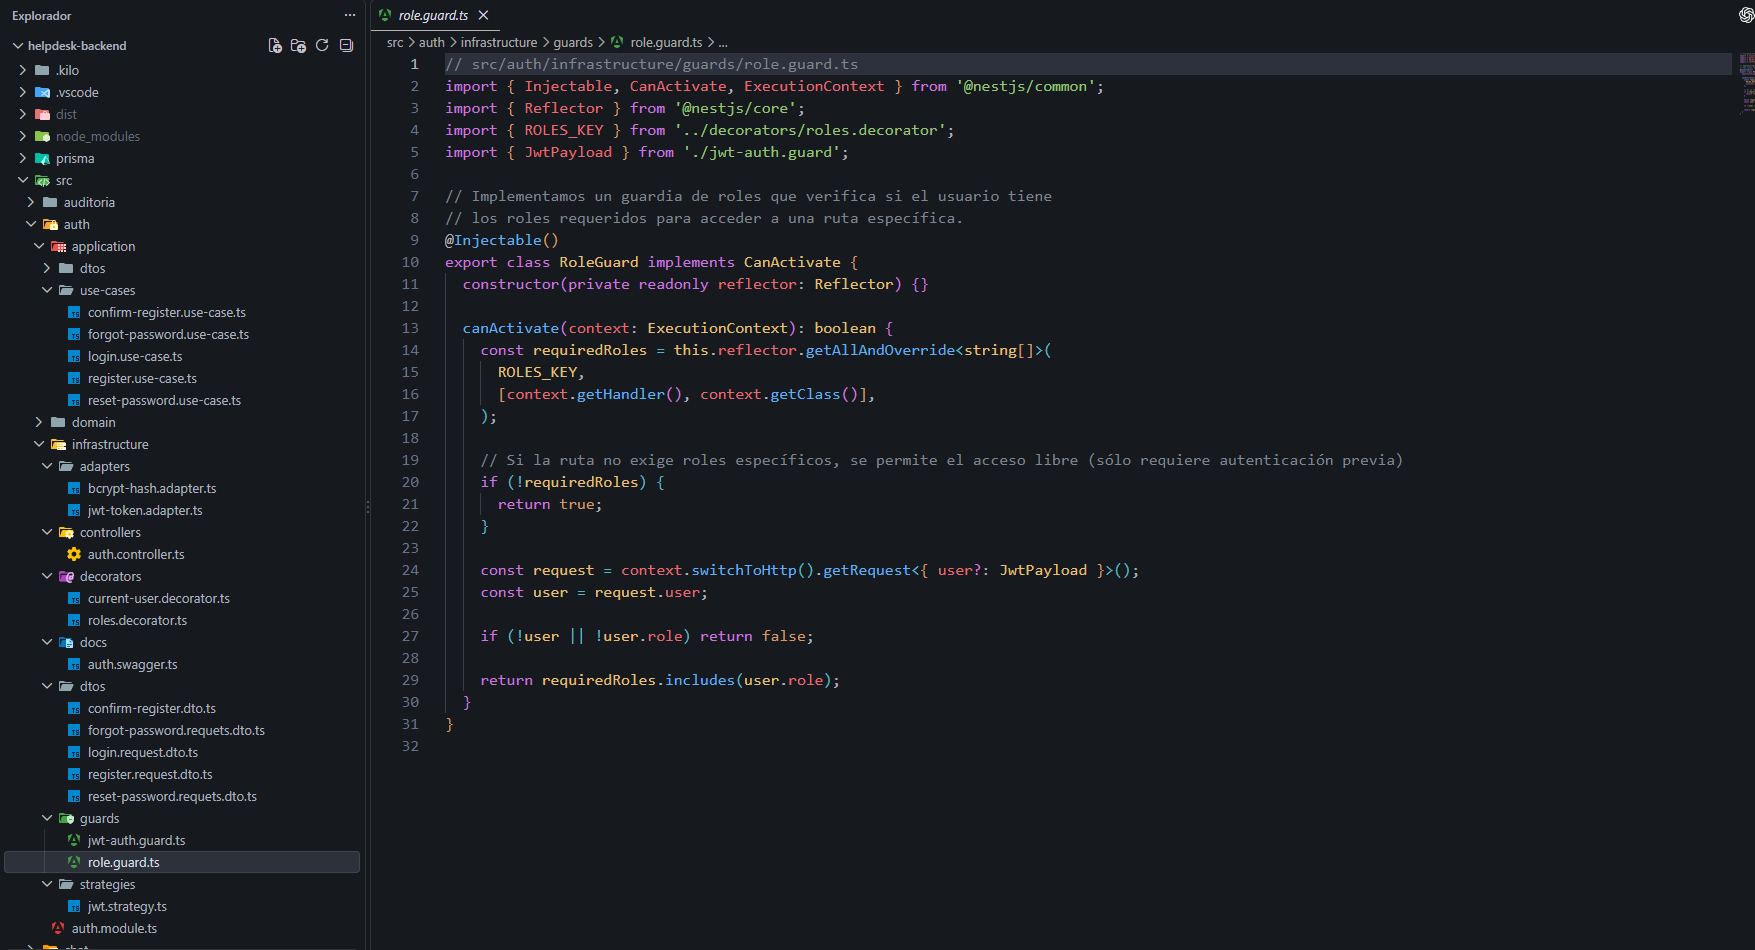
\includegraphics[width=0.92\textwidth]{evidencia_tarea_sprint_2_3.png}
\\[0.2em]
{\small \textit{Nota.} Implementación de controladores, servicios y Guards de seguridad basados en roles (RBAC).}
\end{figure}

\subsubsection{Fase 3: Backend Avanzado, Motor de Asignación y Tiempo Real (Sprint 4)}
Esta fase comprende el desarrollo de la lógica compleja de negocio, integrando el motor de derivación de citas presenciales, comunicación bidireccional mediante WebSockets y caché en Redis, cuyo resumen de actividades se observa en la Tabla \ref{tab:fase3}.

\begingroup
\small
\renewcommand{\arraystretch}{1.25}
\begin{longtable}{@{} p{3.2cm} p{8.8cm} p{3.0cm} @{}}
\caption{{Fase 3: Backend Avanzado, Motor de Asignación y Tiempo Real (Sprint 4)}} \label{tab:fase3} \\
\toprule
\textbf{Actividad / Tarea} & \textbf{Descripción del Entregable} & \textbf{Duración / Plazo} \\
\midrule
\endfirsthead

\multicolumn{3}{@{}l}{\textbf{Tabla \ref{tab:fase3}} \textit{(Continuación)}} \\[0.4em]
\toprule
\textbf{Actividad / Tarea} & \textbf{Descripción del Entregable} & \textbf{Duración / Plazo} \\
\midrule
\endhead

\midrule
\multicolumn{3}{r}{\textit{Continúa en la siguiente página\dots}} \\
\endfoot

\bottomrule
\multicolumn{3}{@{}p{\textwidth}}{\small \textit{Nota.} Actividades correspondientes al desarrollo del motor de citas y comunicación en tiempo real.} \\
\endlastfoot

TR18 - Citas Presenciales & Desarrollo del backend de derivación y gestión de Citas Presenciales. & 5 días \\
TR19 - WebSockets y Redis & Implementación de WebSockets con Redis para Chat y Endpoints de Dashboard. & 6 días \\
\textbf{Total Fase 3} & & \textbf{11 días} \\
\end{longtable}
\endgroup

Como evidencia de esta fase avanzada, se adjuntan el tablero de Jira, el gráfico de seguimiento y la lógica de programación del motor de citas:

\begin{figure}[H]
\centering
\captionsetup{justification=centering}
\caption{Tablero de Jira - Sprint 4 (Motor de Citas y WebSockets)}
\label{fig:evidencia_sprint_4}
\vspace{0.2em}
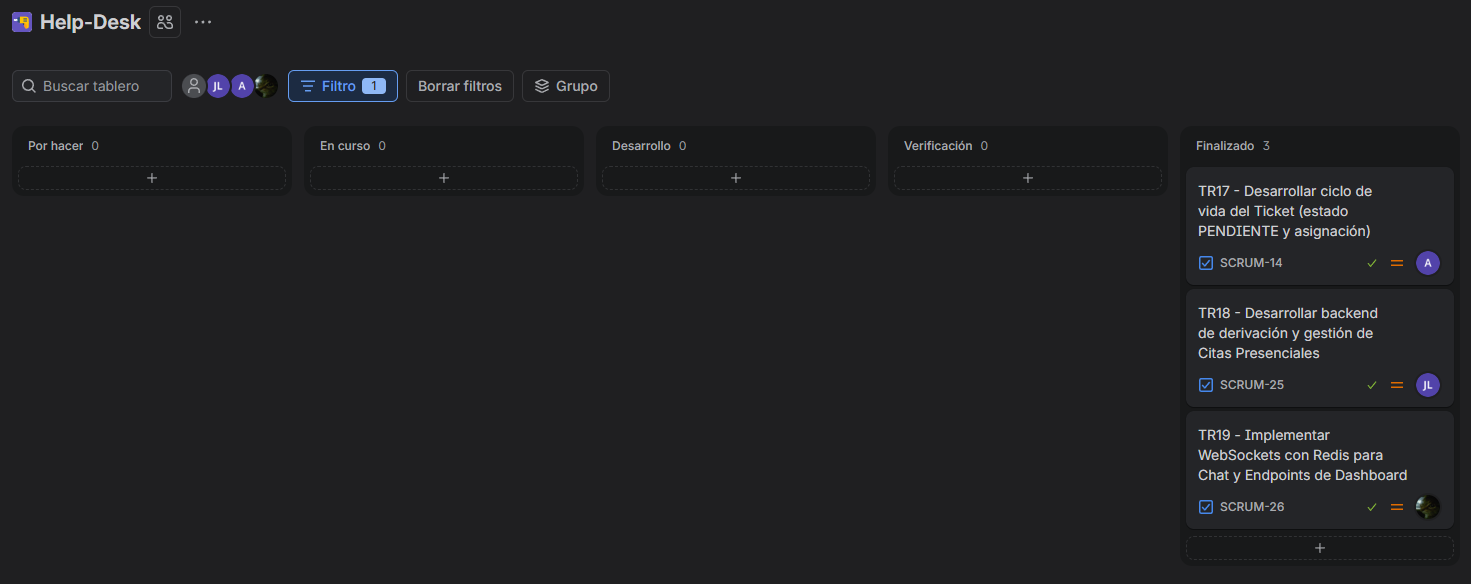
\includegraphics[width=0.92\textwidth]{tablero_sprint_4.png}
\\[0.2em]
{\small \textit{Nota.} Tablero de gestión de tareas para la lógica avanzada de negocio y comunicación en tiempo real.}
\end{figure}

\begin{figure}[H]
\centering
\captionsetup{justification=centering}
\caption{Burndown Chart - Sprint 4}
\label{fig:burndown_sprint_4}
\vspace{0.2em}
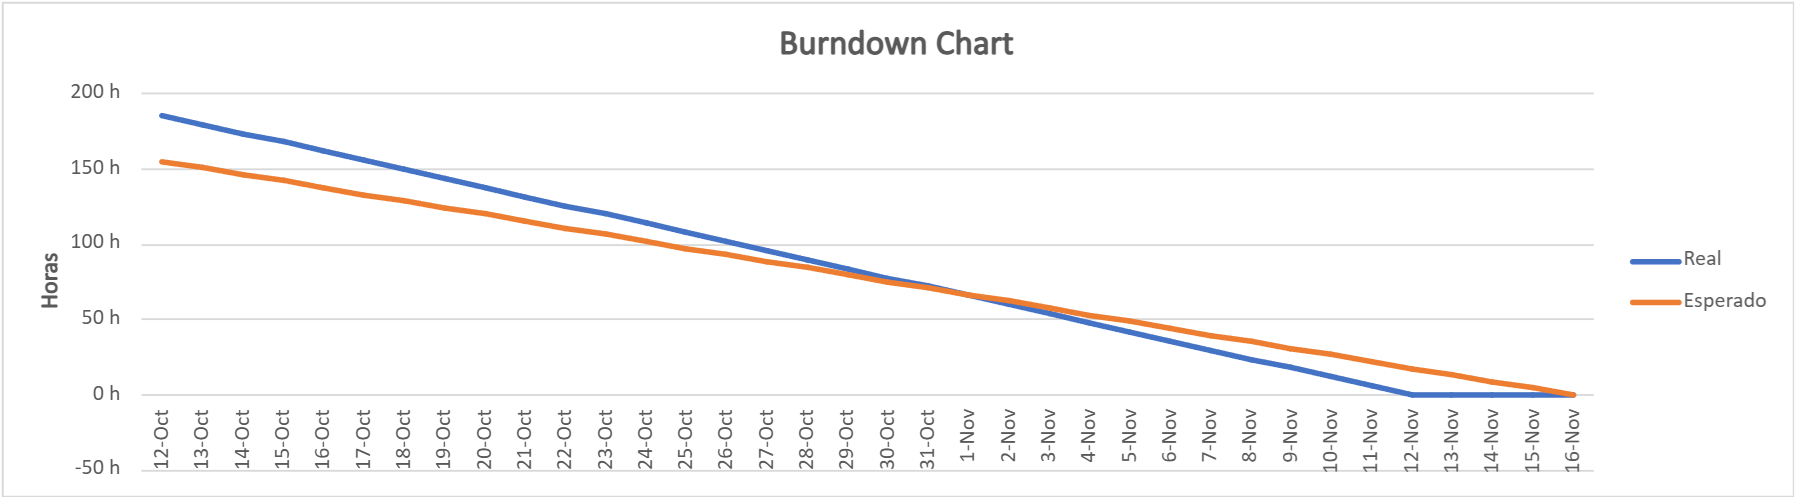
\includegraphics[width=0.92\textwidth]{burdowchart_sprint4.png}
\\[0.2em]
{\small \textit{Nota.} Elaboración propia. Seguimiento de horas estimadas frente al avance real durante el Sprint 4.}
\end{figure}

\begin{figure}[H]
\centering
\captionsetup{justification=centering}
\caption{Evidencia del motor de citas y control anti-cruces}
\label{fig:evidencia_tarea_sprint_4}
\vspace{0.2em}
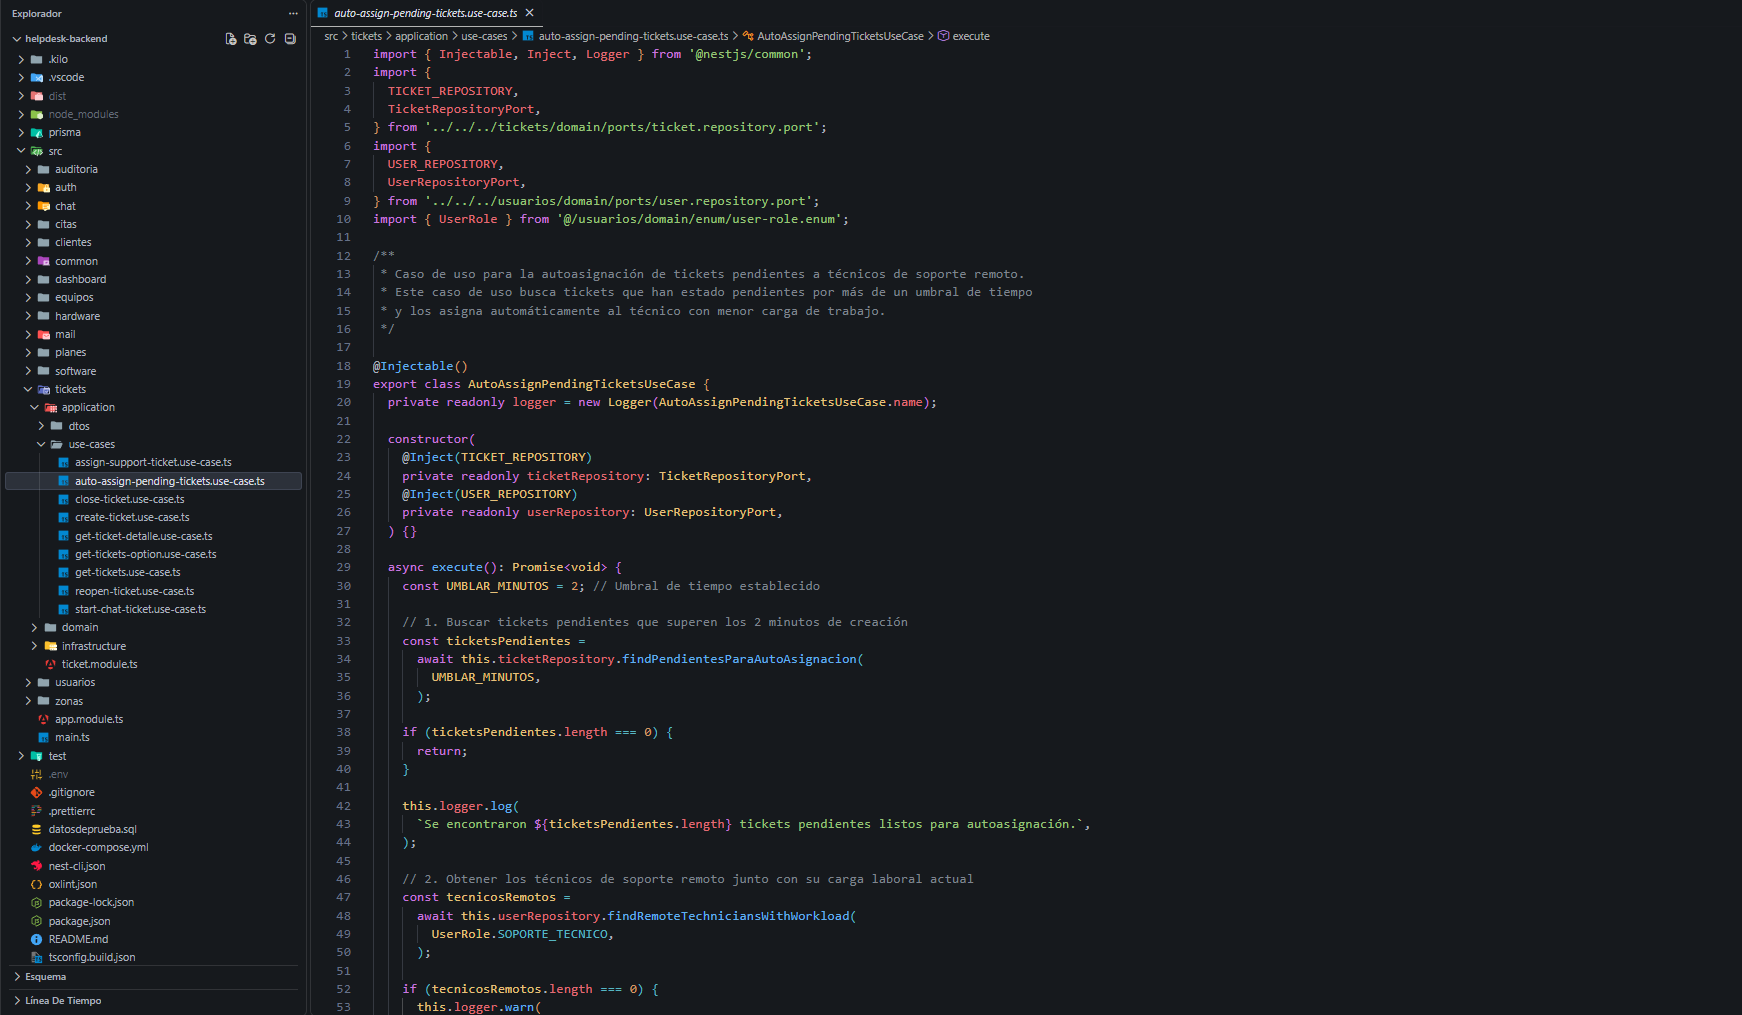
\includegraphics[width=0.92\textwidth]{evidencia_tarea_sprint_4.png}
\\[0.2em]
{\small \textit{Nota.} Implementación del algoritmo de autoasignación por zonas geográficas y gestión de franjas horarias.}
\end{figure}

\subsubsection{Fase 4: Frontend e Interfaces de Usuario (Sprint 5)}
Se enfoca en la implementación del diseño responsivo y la construcción de las pantallas de interacción mediante Next.js y componentes estilizados, estructurando paneles modulares por roles cuyas actividades se reflejan en la Tabla \ref{tab:fase4}.

\begingroup
\small
\renewcommand{\arraystretch}{1.25}
\begin{longtable}{@{} p{3.2cm} p{8.8cm} p{3.0cm} @{}}
\caption{{Fase 4: Frontend e Interfaces de Usuario (Sprint 5)}} \label{tab:fase4} \\
\toprule
\textbf{Actividad / Tarea} & \textbf{Descripción del Entregable} & \textbf{Duración / Plazo} \\
\midrule
\endfirsthead

\multicolumn{3}{@{}l}{\textbf{Tabla \ref{tab:fase4}} \textit{(Continuación)}} \\[0.4em]
\toprule
\textbf{Actividad / Tarea} & \textbf{Descripción del Entregable} & \textbf{Duración / Plazo} \\
\midrule
\endhead

\midrule
\multicolumn{3}{r}{\textit{Continúa en la siguiente página\dots}} \\
\endfoot

\bottomrule
\multicolumn{3}{@{}p{\textwidth}}{\small \textit{Nota.} Tareas de diseño y desarrollo frontend con Next.js y componentes UI.} \\
\endlastfoot

TR20 - Configuración UI & Configuración de estructura modular frontend, Tailwind y componentes UI. & 4 días \\
TR21 - Pantallas Base Frontend & Desarrollo de pantallas frontend de Login, Usuarios y Zonas con \textit{shadcn/ui}. & 6 días \\
TR22 - Jerarquía Organizacional & Desarrollo de interfaces modulares para la Jerarquía Organizacional. & 5 días \\
TR23 - Módulos Operativos & Pantallas de Inventario ITAM, Tickets, Cronograma de Citas, Chat y Dashboard. & 7 días \\
\textbf{Total Fase 4} & & \textbf{22 días} \\
\end{longtable}
\endgroup

Como evidencia del desarrollo frontend, se presentan el tablero, el gráfico de seguimiento y las pantallas principales de la interfaz de usuario:

\begin{figure}[H]
\centering
\captionsetup{justification=centering}
\caption{Tablero de Jira - Sprint 5 (Frontend e Interfaces UI)}
\label{fig:evidencia_sprint_5}
\vspace{0.2em}
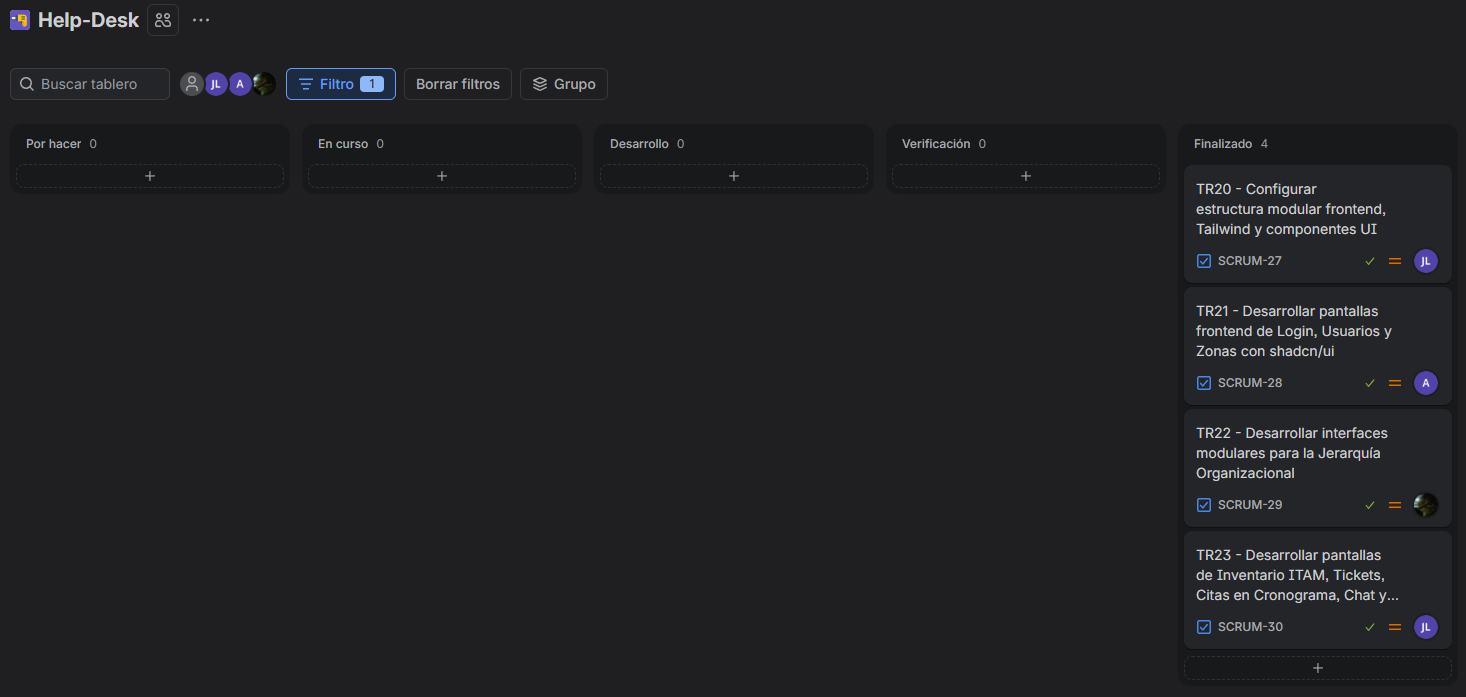
\includegraphics[width=0.92\textwidth]{tablero_sprint_5.png}
\\[0.2em]
{\small \textit{Nota.} Registro de tareas y componentes visuales desarrollados con Next.js y \textit{shadcn/ui}.}
\end{figure}

\begin{figure}[H]
\centering
\captionsetup{justification=centering}
\caption{Burndown Chart - Sprint 5}
\label{fig:burndown_sprint_5}
\vspace{0.2em}
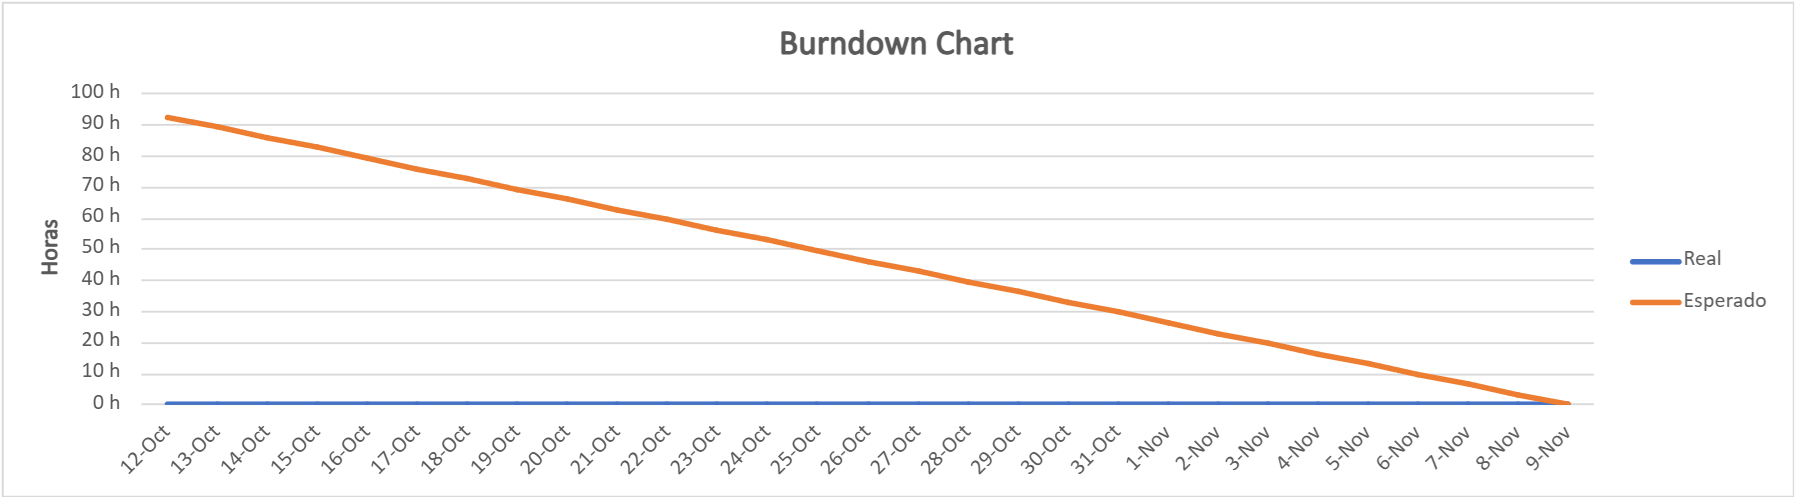
\includegraphics[width=0.92\textwidth]{burdowchart_sprint5.png}
\\[0.2em]
{\small \textit{Nota.} Elaboración propia. Seguimiento de horas estimadas frente al avance real durante el Sprint 5.}
\end{figure}

\begin{figure}[H]
\centering
\captionsetup{justification=centering}
\caption{Vistas operativas principales del sistema frontend (Dashboard - Administrador)}
\label{fig:evidencia_vistas_frontend_1}
\vspace{0.2em}
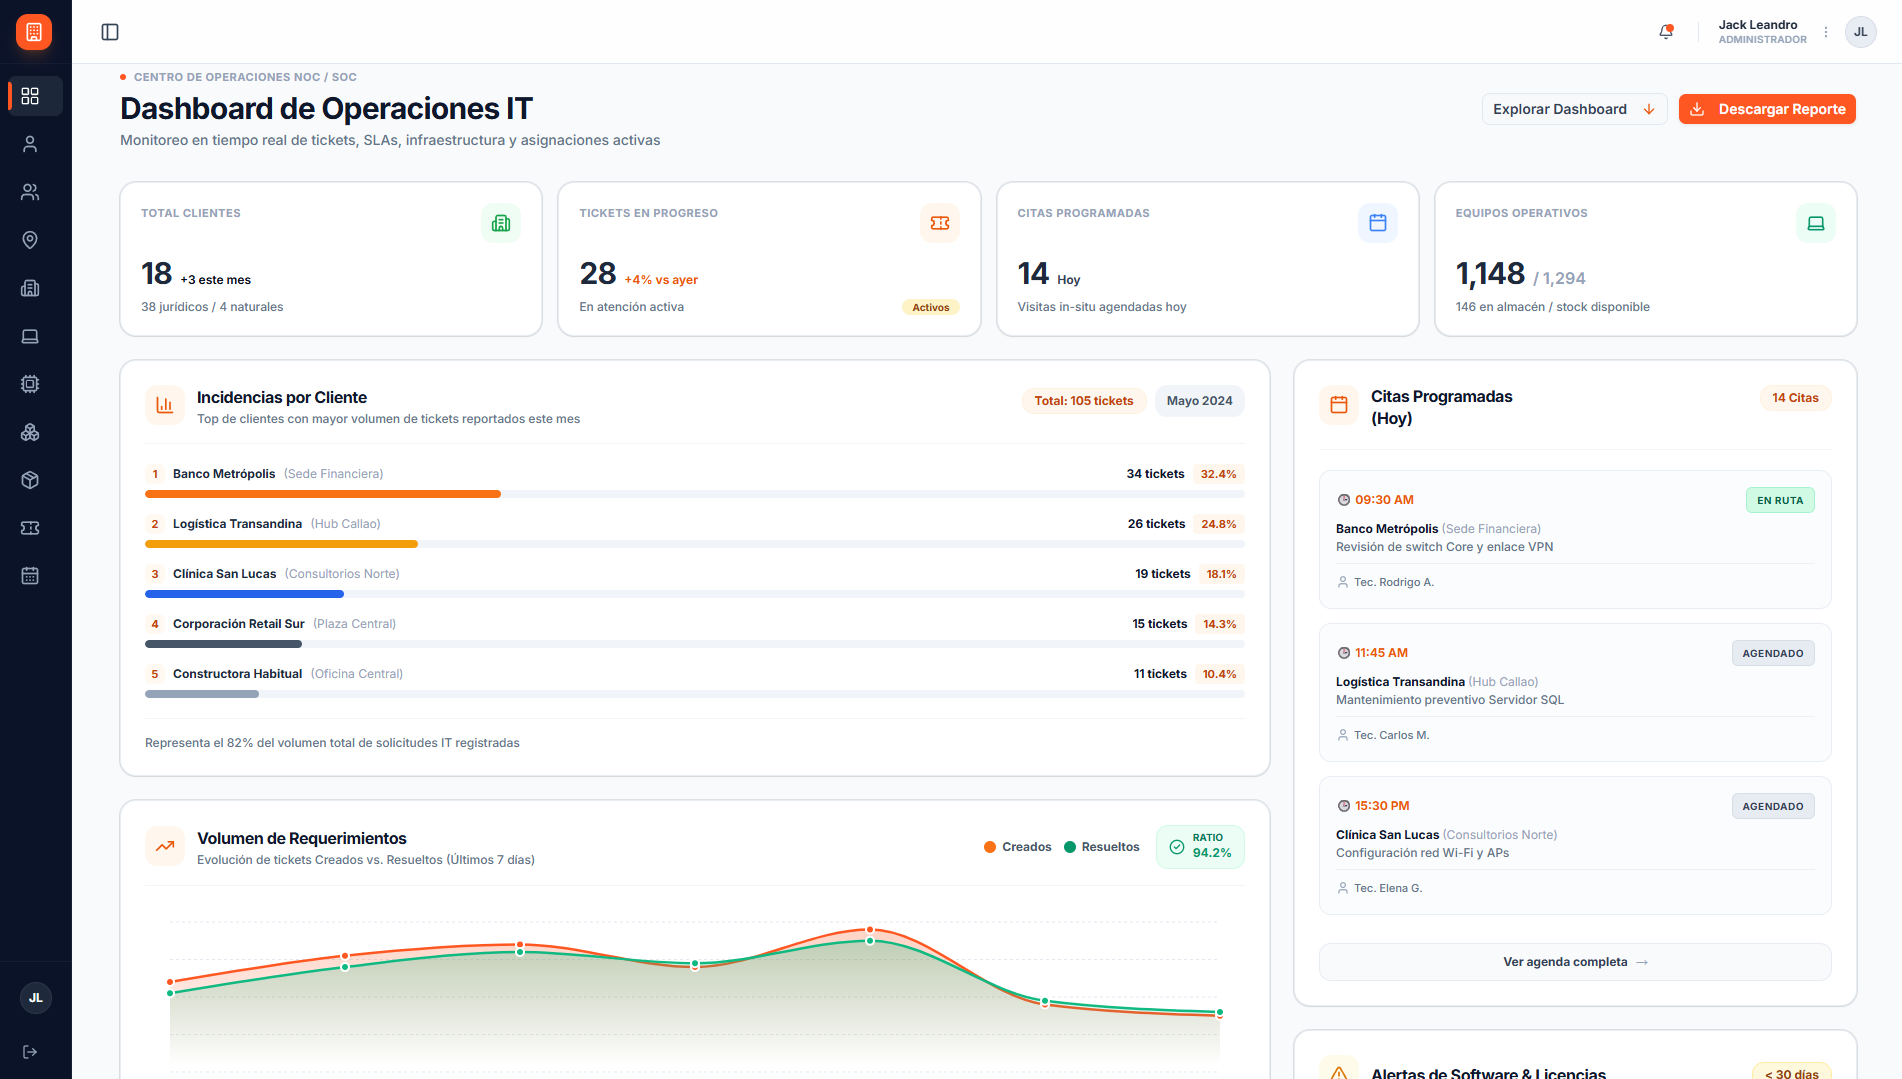
\includegraphics[width=0.92\textwidth]{img/evidencia_frontend_sprint_5_1.png}
\\[0.2em]
{\small \textit{Nota.} Pantallas clave correspondiente al panel de control.}
\end{figure}

\begin{figure}[H]
\centering
\captionsetup{justification=centering}
\caption{Vistas operativas principales del sistema frontend (Módulos Equipos ITAM)}
\label{fig:evidencia_vistas_frontend_2}
\vspace{0.2em}
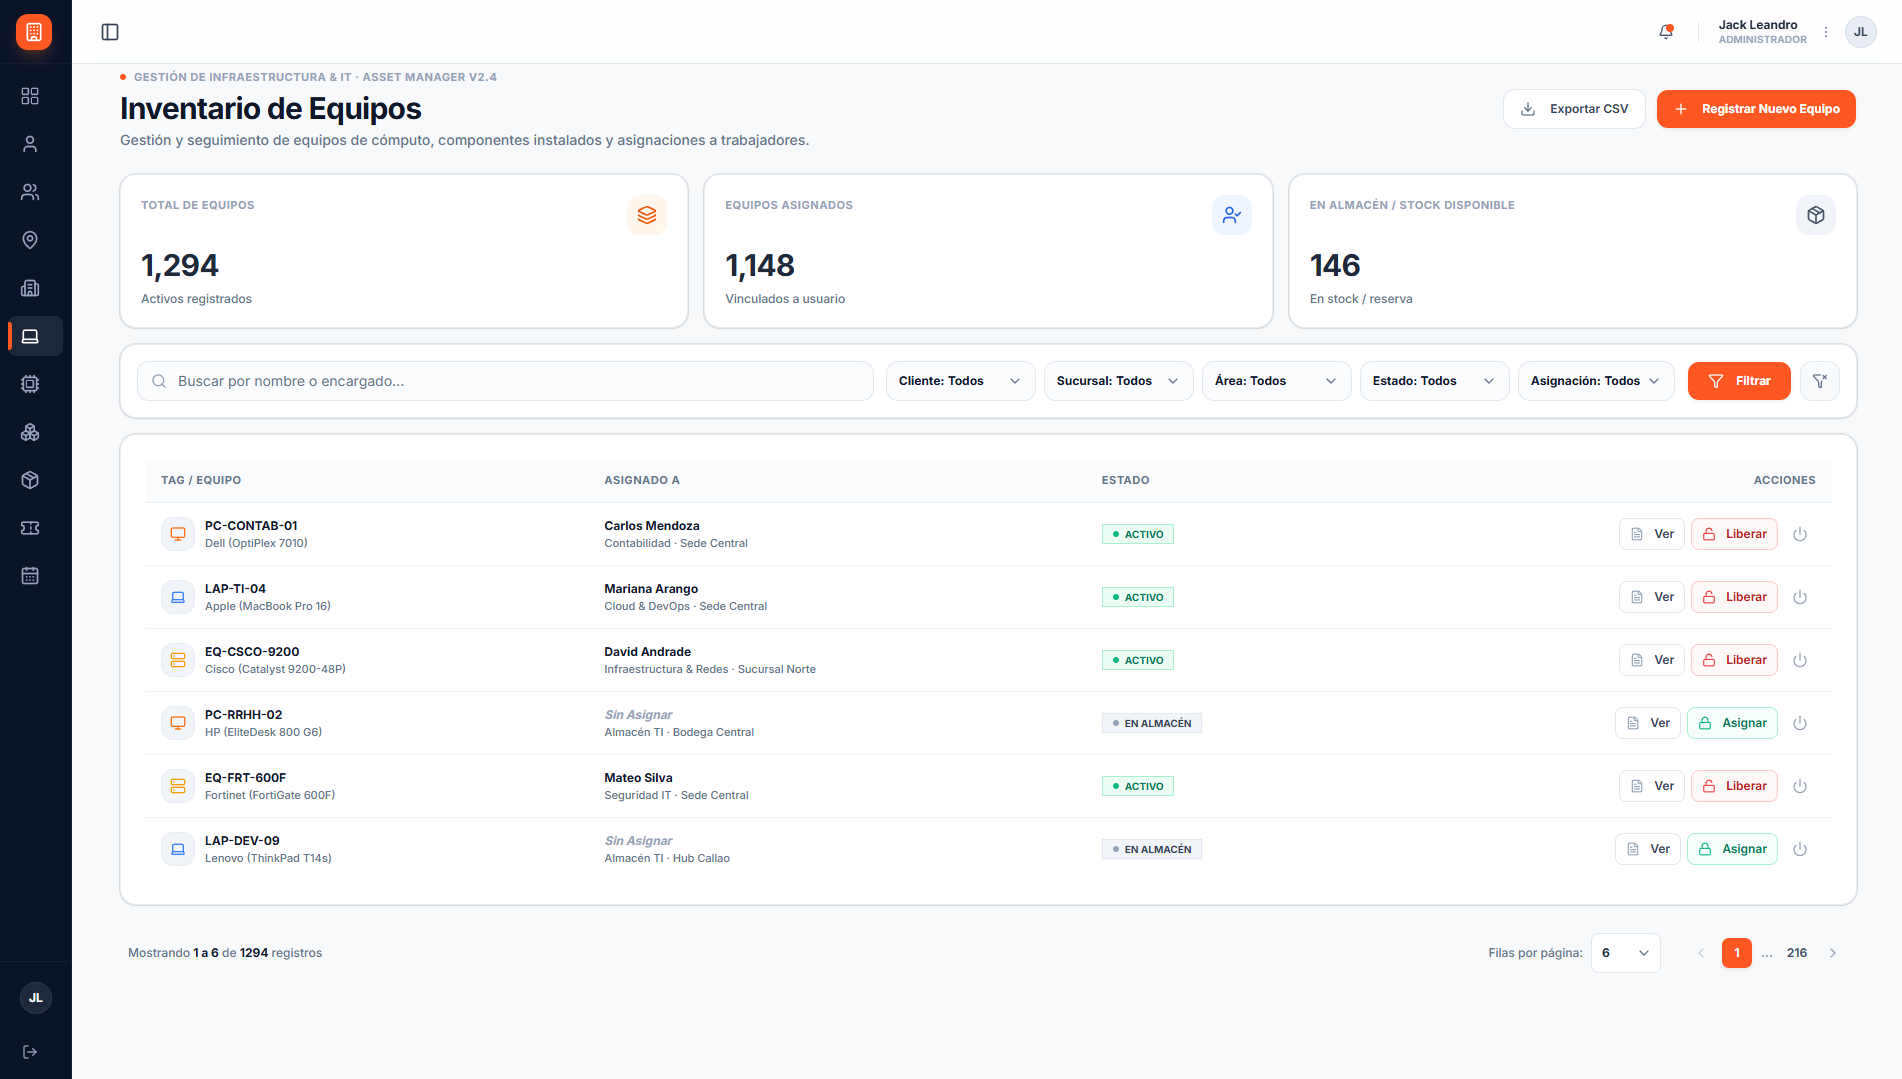
\includegraphics[width=0.92\textwidth]{img/evidencia_frontend_sprint_5_2.png}
\\[0.2em]
{\small \textit{Nota.} Pantallas clave correspondiente a gestión de equipos.}
\end{figure}

\begin{figure}[H]
\centering
\captionsetup{justification=centering}
\caption{Vistas operativas principales del sistema frontend (Módulos ITAM y Tickets)}
\label{fig:evidencia_vistas_frontend_3}
\vspace{0.2em}
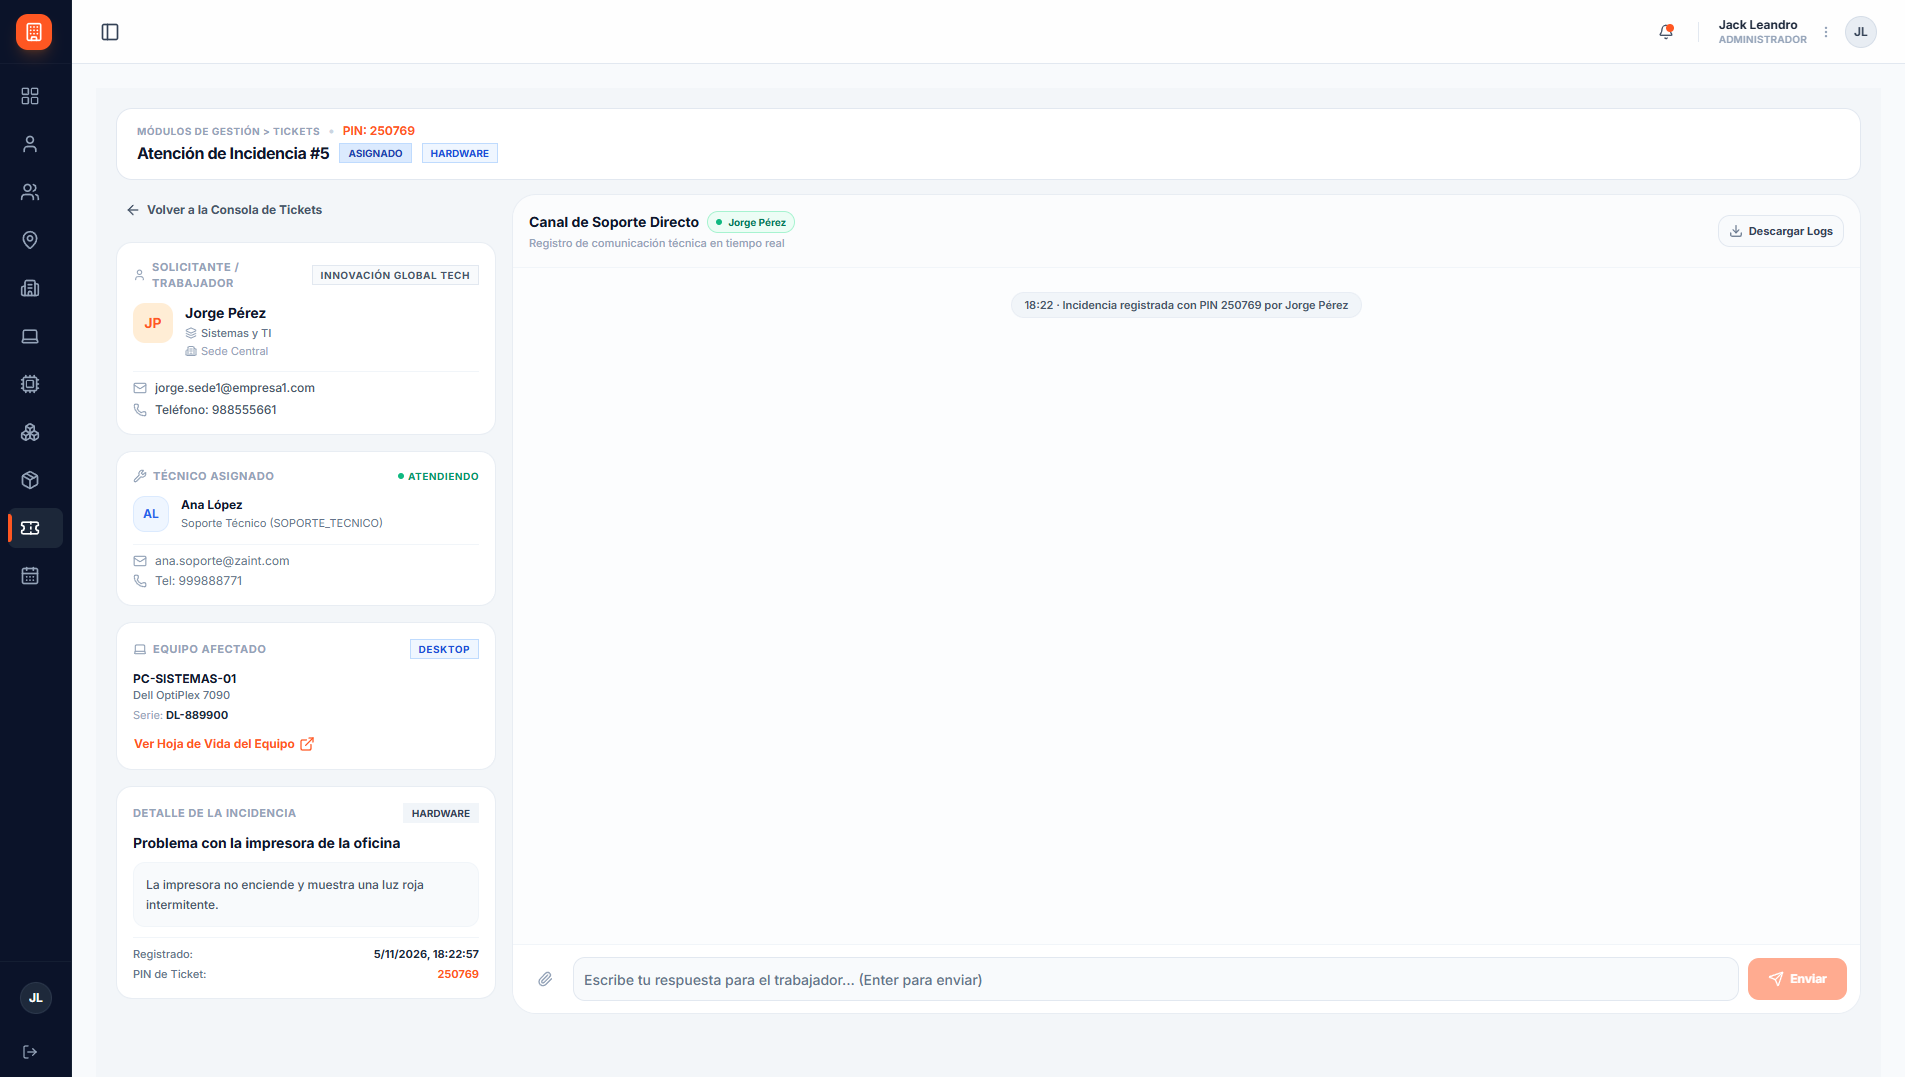
\includegraphics[width=0.92\textwidth]{img/evidencia_frontend_sprint_5_3.png}
\\[0.2em]
{\small \textit{Nota.} Pantallas clave correspondiente al ciclo de vida de ticket.}
\end{figure}

\subsubsection{Fase 5: Calidad, Documentación y Despliegue (Sprint 6)}
Fase final orientada a la validación mediante pruebas unitarias, documentación técnica de endpoints mediante Swagger y la puesta en producción del sistema, cuyas tareas se enumeran en la Tabla \ref{tab:fase5}.

\begingroup
\small
\renewcommand{\arraystretch}{1.25}
\begin{longtable}{@{} p{3.2cm} p{8.8cm} p{3.0cm} @{}}
\caption{{Fase 5: Calidad, Documentación y Despliegue (Sprint 6)}} \label{tab:fase5} \\
\toprule
\textbf{Actividad / Tarea} & \textbf{Descripción del Entregable} & \textbf{Duración / Plazo} \\
\midrule
\endfirsthead

\multicolumn{3}{@{}l}{\textbf{Tabla \ref{tab:fase5}} \textit{(Continuación)}} \\[0.4em]
\toprule
\textbf{Actividad / Tarea} & \textbf{Descripción del Entregable} & \textbf{Duración / Plazo} \\
\midrule
\endhead

\midrule
\multicolumn{3}{r}{\textit{Continúa en la siguiente página\dots}} \\
\endfoot

\bottomrule
\multicolumn{3}{@{}p{\textwidth}}{\small \textit{Nota.} Actividades de pruebas, documentación en Swagger y despliegue en producción.} \\
\endlastfoot

TR24 - Documentación Swagger & Documentación de endpoints y DTOs del Backend usando Swagger. & 4 días \\
TR25 - Pruebas Unitarias Jest & Implementación y ejecución de Pruebas Unitarias en el Backend con Jest. & 5 días \\
TR26 - Módulo de Exportación & Desarrollo de módulo de exportación de documentos PDF. & 5 días \\
TR27 - Despliegue en Producción & Subida de base de datos, backend y frontend al servidor de producción. & 4 días \\
\textbf{Total Fase 5} & & \textbf{18 días} \\
\end{longtable}
\endgroup

Para esta etapa final, se adjunta el tablero de seguimiento actual:

\begin{figure}[H]
\centering
\captionsetup{justification=centering}
\caption{Tablero de Jira - Sprint 6 (En Curso)}
\label{fig:evidencia_sprint_6}
\vspace{0.2em}
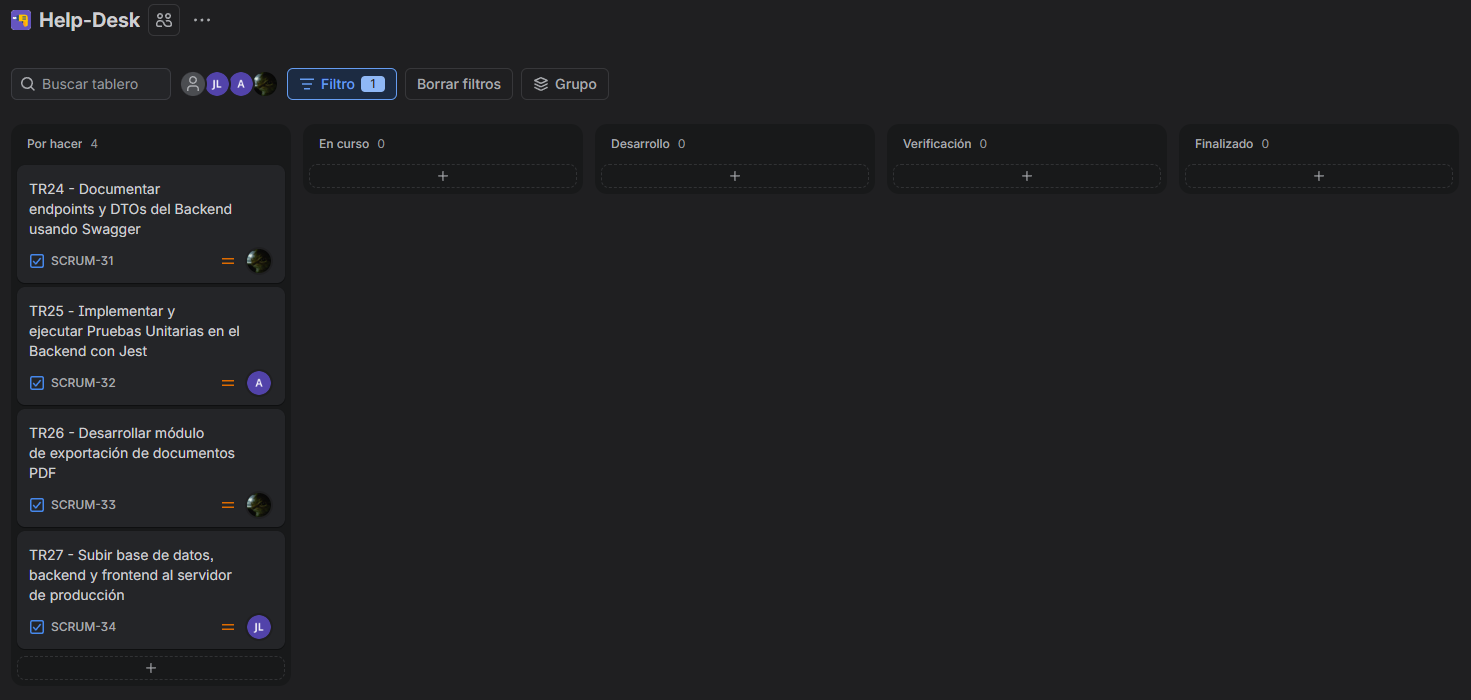
\includegraphics[width=0.92\textwidth]{tablero_sprint_6.png}
\\[0.2em]
{\small \textit{Nota.} Estado actual del tablero para las actividades de documentación en Swagger, pruebas unitarias y despliegue.}
\end{figure}

Nota: Las actividades correspondientes al Sprint 6 se encuentran actualmente en ejecución, abarcando las pruebas de integración finales y la puesta en producción del sistema web.

\section{Consideraciones técnicas, operativas y ambientales para la implementación de la mejora}

\subsection{Consideraciones Técnicas}
La arquitectura de la solución requiere compatibilidad con navegadores web modernos, protocolos de comunicación cifrada mediante HTTPS, autenticación basada en JSON Web Tokens (JWT) y una Arquitectura Modular Basada en Roles en el Frontend. El backend implementa NestJS, TypeScript, MySQL (con Prisma ORM) y Redis para la gestión transaccional y concurrente, aspecto fundamental para garantizar el correcto funcionamiento del algoritmo de reservas temporales (\textit{SoftLock}) y la autoasignación concurrente de citas.

\subsection{Consideraciones Operativas}
La puesta en marcha de la plataforma demanda una transición ordenada desde los canales informales (chats de WhatsApp, llamadas telefónicas) y registros dispersos en hojas de cálculo hacia el sistema Web Help-Desk centralizado. Esto optimiza de forma directa la operación diaria de la empresa J\&P Periféricos S.A.C. mediante los siguientes ejes operativos:

\begin{itemize}
\item \textbf{Formalización del Ingreso de Solicitudes:} Los usuarios finales ya no reportarán fallas por vías informales u opacas; cada incidencia generará formalmente un ticket de soporte asociado a un código PIN único, garantizando un registro centralizado y trazable.

\item \textbf{Inventario TI Centralizado y Hoja de Vida de Equipos:} El sistema integra la gestión detallada del parque informático corporativo organizado por empresas cliente, sucursales y áreas. Esto permite a los equipos de soporte consultar en tiempo real la \textbf{hoja de vida técnica} de cada equipo (historial de fallas, hardware instalado y licencias de software asignadas), brindando el contexto técnico necesario para agilizar la resolución de incidencias.

\item \textbf{Algoritmo Automatizado de Autoasignación y Derivación In-Situ:} 
El flujo operativo distingue claramente entre la atención remota y presencial:
\begin{itemize}
    \item Cuando el soporte remoto determina que la falla no puede resolverse de forma virtual, ejecuta la derivación hacia soporte presencial (\textit{in-situ}).
    \item El algoritmo de autoasignación analiza de forma automatizada los técnicos disponibles filtrando por la \textbf{zona geográfica de la sucursal}.
    \item Adicionalmente, el motor inteligente verifica si el técnico seleccionado ya cuenta con citas agendadas en la \textbf{misma sucursal}, priorizando y asignando esa misma franja horaria para agrupar hasta un máximo de tres (3) atenciones presenciales en una sola visita. Esto elimina desplazamientos innecesarios y optimiza los tiempos de traslado del personal técnico.
\end{itemize}

\item \textbf{Gestión de Componentes y Credenciales en Campo:} Durante las visitas presenciales, el técnico de soporte \textit{in-situ} gestiona dinámicamente la hoja de vida del equipo. Si se realiza el reemplazo o instalación de un nuevo componente de hardware (discos, memorias, etc.), el sistema registra la modificación de forma inmediata. Asimismo, el técnico cuenta con acceso controlado a las credenciales y claves de licencias de software requeridas para la intervención.

\item \textbf{Gestión del Cambio y Capacitación:} Se estructurará un plan de capacitación adaptado a cada perfil: inducción rápida para trabajadores finales (apertura de tickets), entrenamiento operativo para técnicos (gestión de hoja de vida y derivaciones), y uso de reportes y tableros métricos para la administración.

\end{itemize}

\subsection{Consideraciones Ambientales}
La implementación del sistema aporta beneficios directos desde la perspectiva ambiental y el desarrollo sostenible de las operaciones tecnológicas:
\begin{itemize}
\item \textbf{Reducción del Consumo de Papel y Suministros:} La digitalización integral del ciclo de vida de los tickets y los expedientes técnicos de hardware/software elimina drásticamente el uso de formularios físicos, cuadernos de registro manual e impresiones innecesarias de informes técnicos.
\item \textbf{Optimización de Desplazamientos y Menor Huella de Carbono:} Gracias al motor automatizado de asignación y agrupación de citas presenciales por zonas geográficas, se evitan viajes duplicados o traslados ineficientes del personal técnico. Esto disminuye el consumo de combustible de las unidades de transporte y reduce las emisiones de gases de efecto invernadero asociadas a la logística de campo.
\item \textbf{Eficiencia Energética en Infraestructura Digital:} Al centralizar los servicios sobre una arquitectura web optimizada (con gestión eficiente de consultas mediante caché en Redis), se reduce la sobrecarga de procesamiento local en equipos, promoviendo un menor consumo de energía eléctrica y prolongando la vida útil del parque informático de la empresa.
\end{itemize}

\section{Recursos técnicos para la implementación de la mejora}

Para garantizar el correcto desarrollo, despliegue y funcionamiento del sistema Web Help-Desk centralizado, se han estructurado los recursos técnicos en tres categorías esenciales:

\subsection{Infraestructura de Servidores y Conectividad}
\begin{itemize}
\item \textbf{Servidor de Alojamiento (Hosting):} Entorno de producción virtualizado en la nube con alta disponibilidad para hospedar los servicios del backend y frontend.
\item \textbf{Dominio y Protocolo SSL:} Dominio web propio con certificado de seguridad HTTPS para garantizar conexiones cifradas y proteger la integridad de los datos institucionales.
\item \textbf{Gestor de Mensajería en Tiempo Real:} Servidor Redis configurado para el manejo de canales de caché y soporte de eventos mediante WebSockets en las notificaciones y chats de soporte.
\end{itemize}

\subsection{Entorno de Desarrollo Software y Herramientas Tecnológicas}
\begin{itemize}
\item \textbf{Entorno Backend y Lenguaje:} Node.js como motor de ejecución y TypeScript como lenguaje tipado para el desarrollo de la API.
\item \textbf{Framework de Arquitectura:} NestJS estructurado bajo un enfoque modular y principios de código limpio.
\item \textbf{Entorno Frontend:} Next.js con Arquitectura Modular Basada en Roles para interfaces responsivas y dinámicas.
\item \textbf{Gestión de Bases de Datos:} MySQL para datos transaccionales mediante Prisma ORM, y MongoDB para el almacenamiento no relacional del historial de auditoría e interacciones.
\item \textbf{Control de Versiones y Documentación:} Git para la trazabilidad del código fuente y Swagger UI para la documentación interactiva de los endpoints.
\end{itemize}

\subsection{Hardware de Soporte y Estaciones de Trabajo}
\begin{itemize}
\item \textbf{Equipos de Computación:} Computadoras portátiles con procesadores de alto rendimiento, memoria RAM ampliada y discos de estado sólido (SSD) destinados a la codificación, compilación y pruebas locales del software.
\end{itemize}

\section{Diagrama del proceso, mapa del flujo de valor y/o diagrama de operación de la situación mejorada}
\subsection{Proceso de la empresa con la intervención del software}
Con la implementación de la solución tecnológica y el motor automatizado, el flujo de operaciones del área experimenta una automatización integral, reduciendo los tiempos de respuesta y centralizando las solicitudes de manera segura.

A continuación, se presentan los diagramas de procesos detallados por carriles (\textit{swimlanes}), redactados bajo notación de verbos en infinitivo y estructurados según el control de acceso basado en roles (RBAC) y la arquitectura multinivel del sistema:

\subsection{Proceso de Consulta de Hoja de Vida de Equipos (ITAM)}

El proceso de consulta de la hoja de vida de un activo informático permite la trazabilidad completa del historial de mantenimientos, componentes instalados y licencias asociadas. El acceso está determinado por el alcance del rol del usuario autenticado (Trabajador, Sucursal, Empresa o Soporte), garantizando que cada perfil consulte únicamente la información que le corresponde.

\begin{figure}[H]
\centering
\captionsetup{justification=centering}
\caption{Proceso de Consulta de Hoja de Vida de Equipos (ITAM)}
\label{fig:proceso_consulta_itam}
\vspace{0.2em}
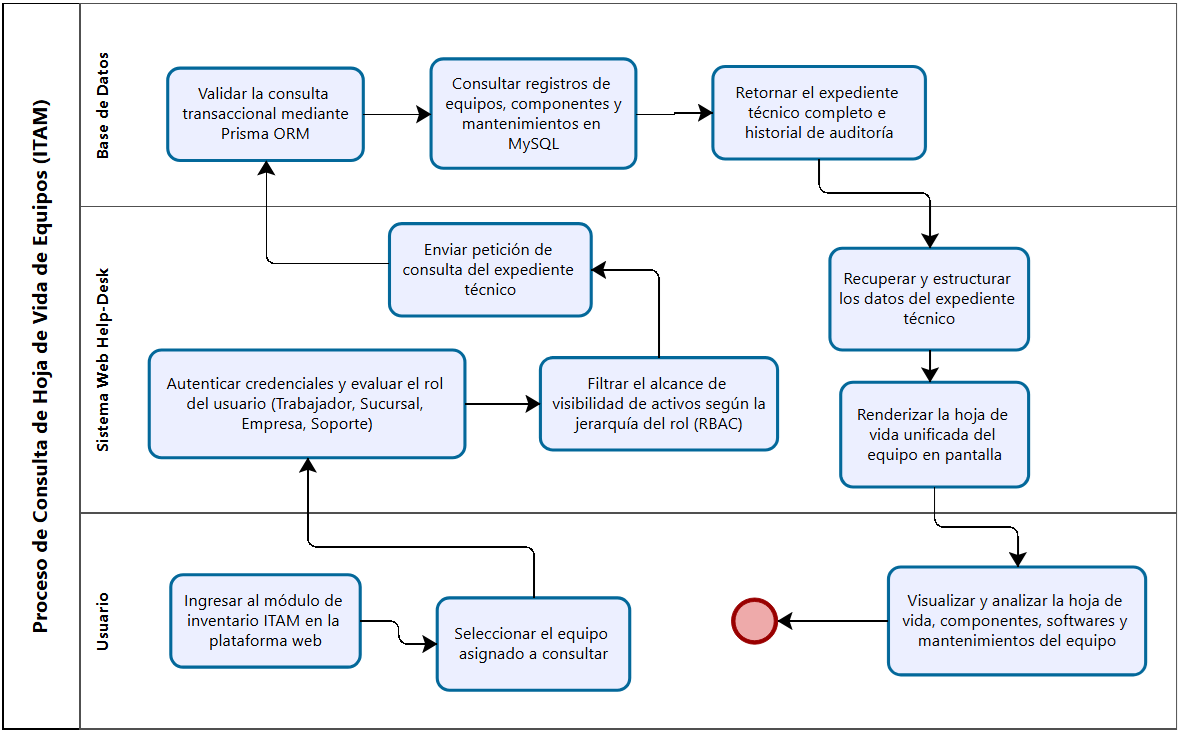
\includegraphics[width=0.92\textwidth]{Proceso de Consulta de Hoja de Vida de Equipos (ITAM).png}
\\[0.2em]
{\small \textit{Nota.} Esquema del flujo de consulta con filtrado de visibilidad por alcance de rol (RBAC) y respuesta transaccional mediante Prisma ORM.}
\end{figure}

\subsection{Proceso de Gestión y Registro de Hardware (ITAM)}

La administración física de los dispositivos tecnológicos contempla dos mecanismos principales de ingreso: el alta unitaria de componentes o equipos y la importación masiva por lotes mediante plantillas estandarizadas de Excel.

\begin{figure}[H]
\centering
\captionsetup{justification=centering}
\caption{Proceso de Gestión y Registro de Hardware (ITAM)}
\label{fig:proceso_gestion_hardware}
\vspace{0.4em}

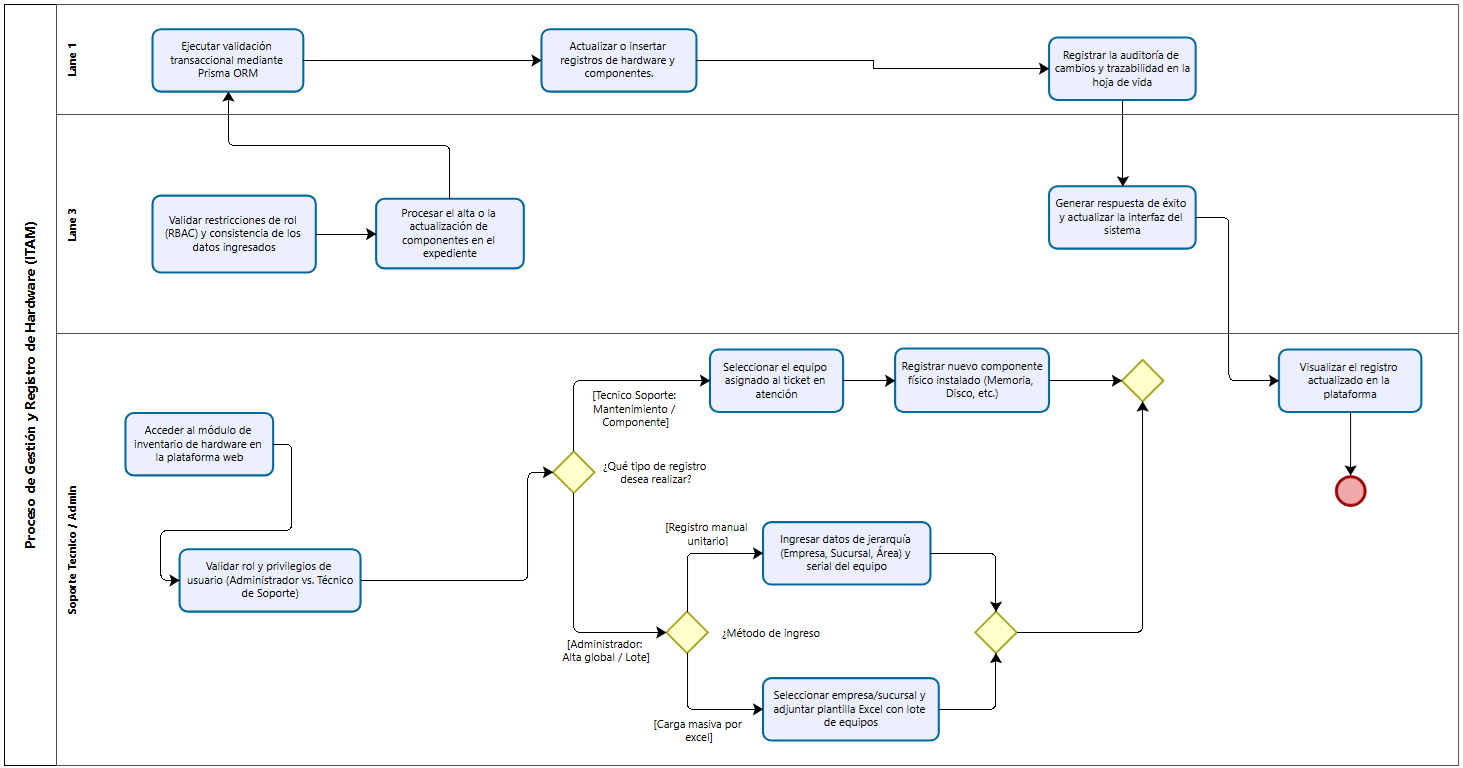
\includegraphics[width=0.95\textwidth]{Proceso de Gestión y Registro de Hardware (ITAM).png}

\vspace{0.4em}
{\small \textit{Nota.} Flujo de decisión entre registro unitario, carga por lote en Excel y mantenimiento por el técnico de soporte.}

\end{figure}

\subsection{Proceso de Gestión de Software y Licencias (ITAM)}

La gestión del catálogo de aplicaciones corporativas y asignación de licencias requiere un control riguroso del stock disponible para evitar sobrecostos o usos no autorizados.

\begin{figure}[H]
\centering
\captionsetup{justification=centering}
\caption{Proceso de Gestión de Software y Licencias (ITAM)}
\label{fig:proceso_gestion_software}
\vspace{0.4em}

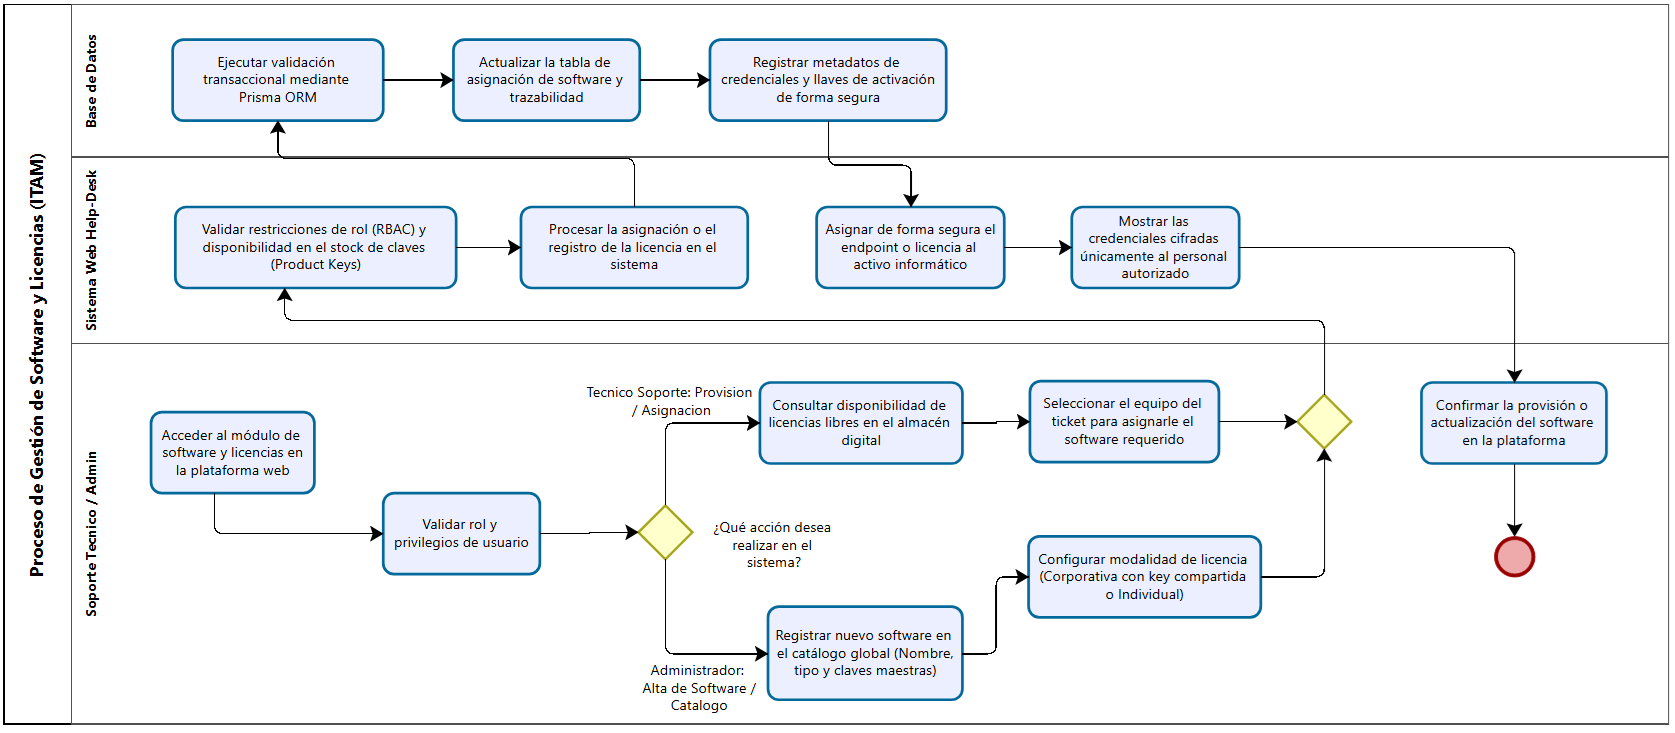
\includegraphics[width=0.95\textwidth]{Proceso de Gestión de Software y Licencias (ITAM).png}

\vspace{0.4em}
{\small \textit{Nota.} Representación del alta en el catálogo global y la asignación de claves de activación al activo correspondiente.}

\end{figure}

\subsection{Proceso de Gestión de Tickets y Soporte Técnico Remoto}

El flujo principal de atención remota ante incidencias tecnológicas inicia con la solicitud formal emitida por el trabajador, asignando de forma automatizada a un técnico disponible y ofreciendo comunicación directa.

\begin{figure}[H]
\centering
\captionsetup{justification=centering}
\caption{Proceso de Gestión de Tickets y Soporte Técnico Remoto}
\label{fig:proceso_tickets_soporte_remoto}
\vspace{0.4em}

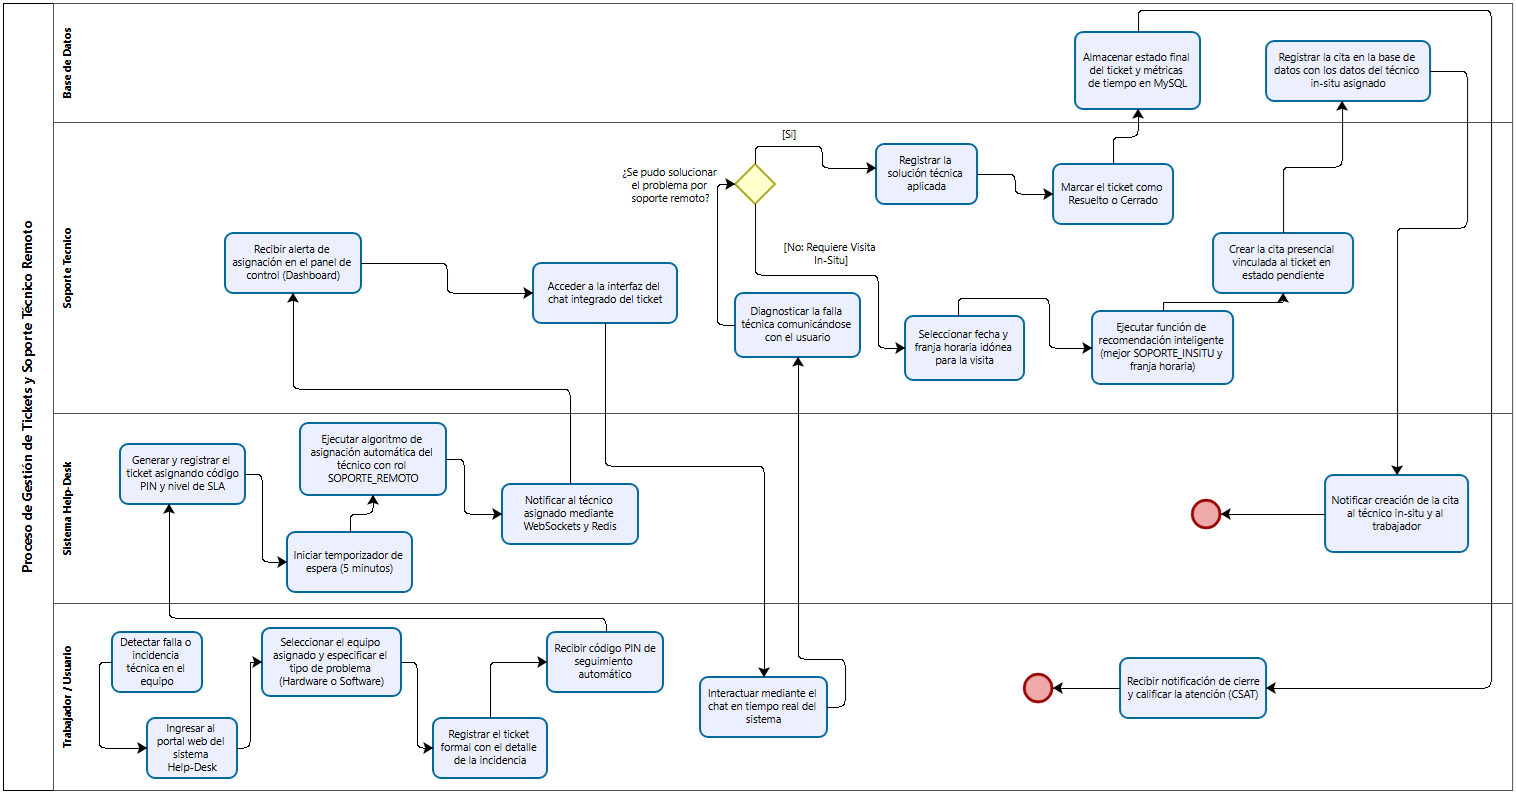
\includegraphics[width=0.95\textwidth]{Proceso de Gestión de Tickets y Soporte Técnico Remoto.png}

\vspace{0.4em}
{\small \textit{Nota.} Flujo transaccional desde el registro del ticket, la atención vía WebSockets y la derivación inteligente a soporte in-situ.}

\end{figure}

\subsection{Proceso de Soporte In-Situ y Ciclo de Vida de la Cita}

Para aquellas incidencias que demandan intervención física en las instalaciones de la empresa cliente, el sistema gestiona la asignación y el ciclo de estados de la visita presencial.

\begin{figure}[H]
\centering
\captionsetup{justification=centering}
\caption{Proceso de Soporte In-Situ y Ciclo de Vida de la Cita}
\label{fig:proceso_soporte_insitu}
\vspace{0.4em}

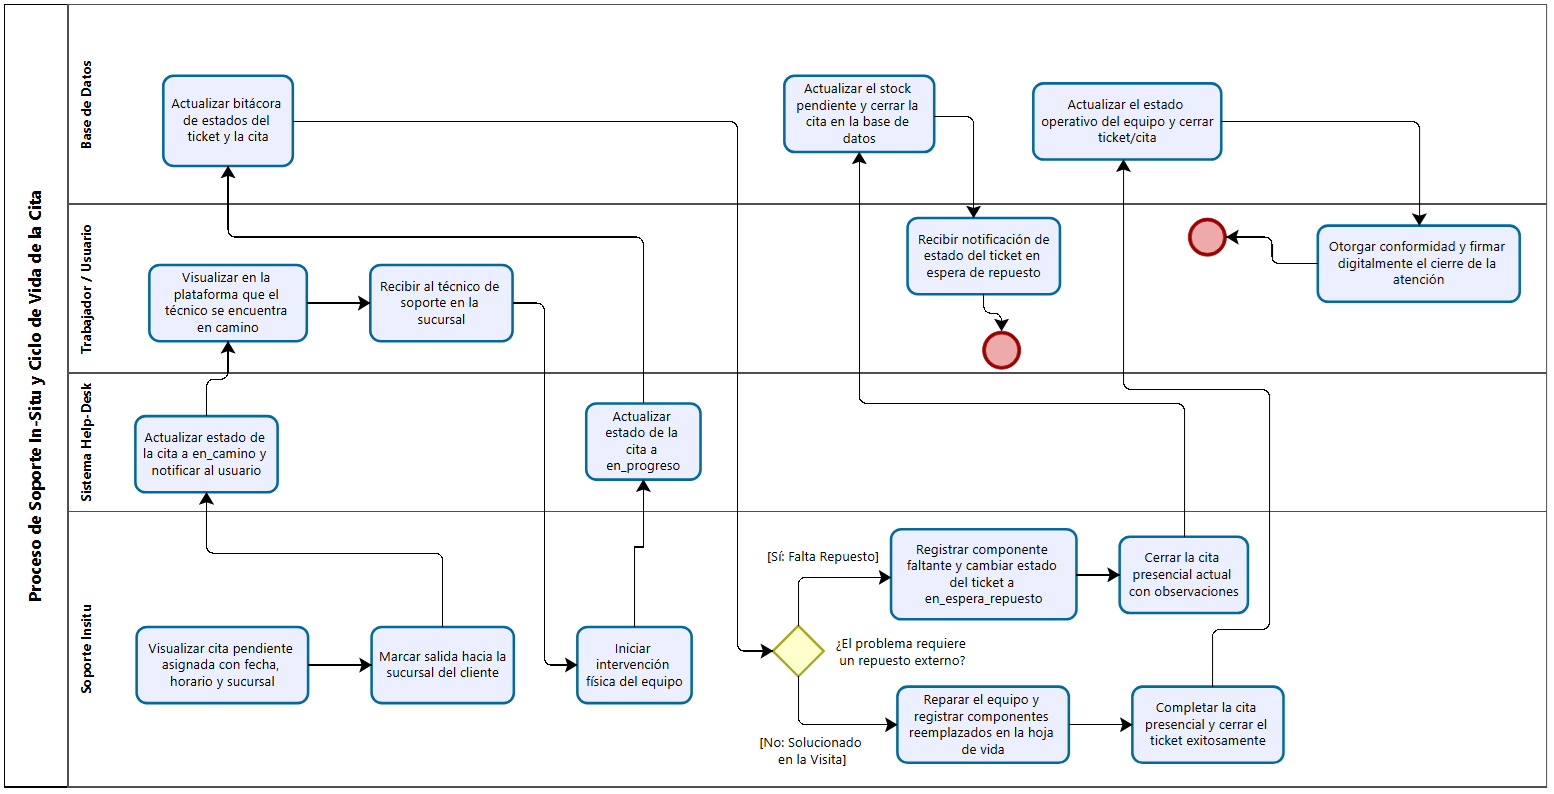
\includegraphics[width=0.95\textwidth]{Proceso de Soporte In-Situ y Ciclo de Vida de la Cita.png}

\vspace{0.4em}
{\small \textit{Nota.} Ciclo de vida de la cita presencial y atención según los escenarios de solución inmediata o espera de repuestos.}

\end{figure}

\section{Cronograma de ejecución de la mejora}
La ejecución del proyecto se proyecta en un período estructurado conforme al avance de los sprints de desarrollo:
\begin{enumerate}
\item \textbf{Sprint 1:} Análisis de requerimientos y diseño de arquitectura base (Prisma, entidades y roles).
\item \textbf{Sprint 2:} Desarrollo del backend, conexiones a base de datos, lógica de negocio, motor de autoasignación por zona y carga, y seguridad JWT.
\item \textbf{Sprint 3:} Desarrollo del frontend (Next.js), interfaces de usuario y paneles de control con arquitectura modular por roles, tableros Kanban y gestión de citas con \textit{SoftLock}.
\item \textbf{Sprint 4:} Pruebas de integración, validación de flujos de derivación, corrección de errores y despliegue final en producción.
\end{enumerate}

\newpage

A continuación, se presenta el diagrama de Gantt que detalla la planificación y el estado actual de las tareas del proyecto:

\begin{figure}[H]
\centering
\captionsetup{justification=centering}
\caption{Cronograma de Ejecución y Planificación del Proyecto (Parte 1)}
\label{fig:cronograma_ejecucion_1}
\vspace{0.3em}

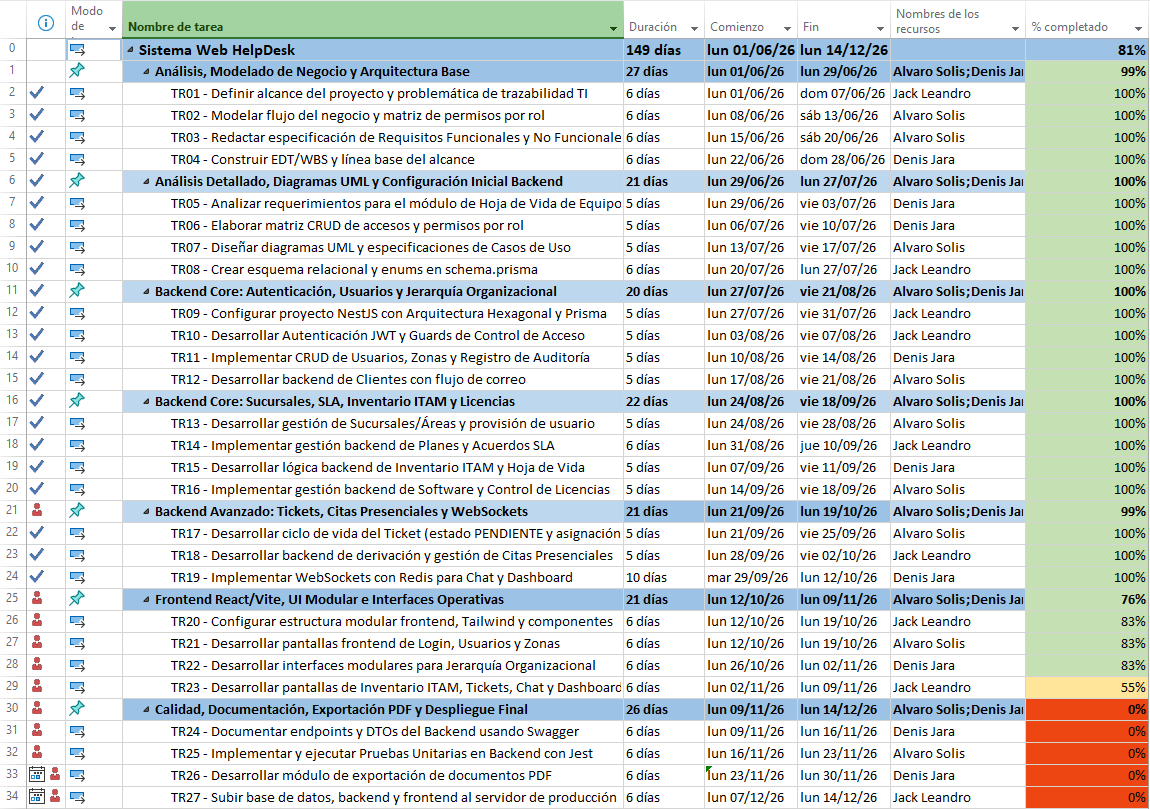
\includegraphics[width=0.98\textwidth, trim=0 0 0 0, clip]{Cronograma-Proyecto-1.png}

\vspace{-0.4em}
{\small \textit{Nota.} Elaboración propia basada en la planificación del sistema Help-Desk centralizado en Microsoft Project. Primera parte del cronograma.}

\end{figure}

\begin{figure}[H]
\centering
\captionsetup{justification=centering}
\caption{Cronograma de Ejecución y Planificación del Proyecto (Parte 2)}
\label{fig:cronograma_ejecucion_2}
\vspace{0.3em}

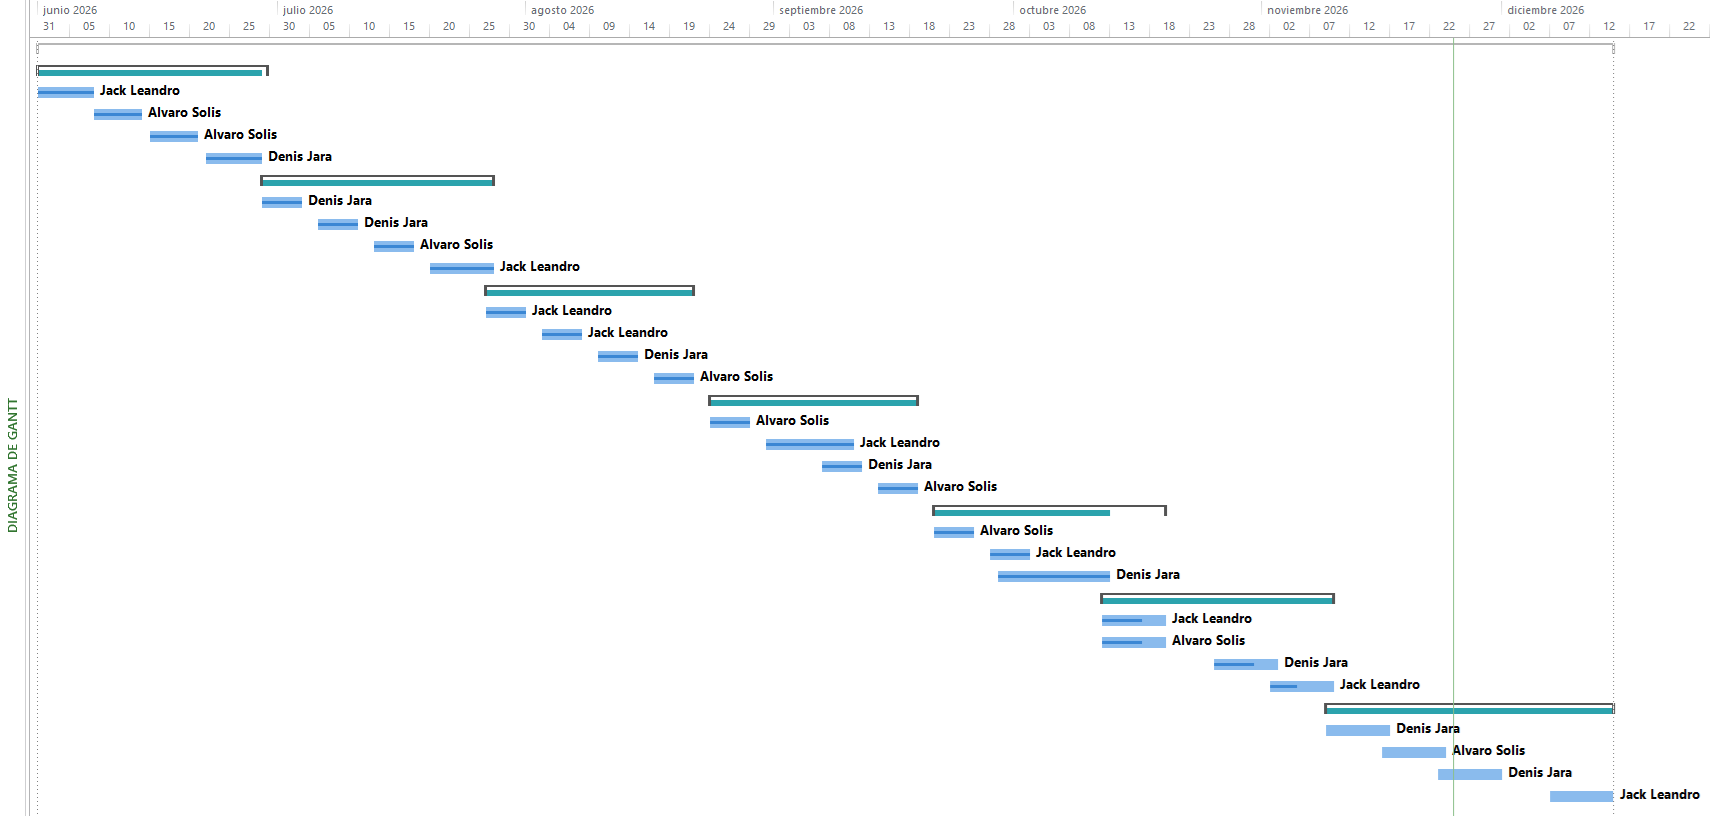
\includegraphics[width=0.98\textwidth, trim=0 0 0 0, clip]{Cronograma-Proyecto-2.png}

\vspace{-0.4em}
{\small \textit{Nota.} Elaboración propia basada en la planificación del sistema Help-Desk centralizado en Microsoft Project. Segunda parte del cronograma.}

\end{figure}

Como se observa en la figura, el porcentaje de completado de las tareas está representado mediante una escala de colores en la columna correspondiente. El \textbf{color verde oscuro} indica las fases y tareas concluidas al 100\% (valor máximo), correspondientes a la arquitectura base, desarrollo del backend y la mayor parte del frontend. El \textbf{color amarillo} denota una tarea en curso con un avance parcial del 66\% (correspondiente a pantallas de inventario ITAM, tickets, chat y dashboard). Por último, el \textbf{color rojo} señala las actividades pendientes con un avance del 0\%, vinculadas a la fase final de control de calidad, exportación PDF y despliegue en producción.

\newpage

\section{Aspecto limitante para la implementación de la mejora}
Durante el proceso de implantación y puesta en marcha de la solución tecnológica centralizada, se han identificado diversos factores limitantes de carácter técnico, operativo y organizacional que podrían influir en la adopción del sistema. Estos aspectos se clasifican y detallan a continuación según los actores involucrados:

\begin{itemize}
\item \textbf{Limitaciones asociadas a la empresa (J\&P Periféricos S.A.C. - JYP) y su infraestructura tecnológica:}
\begin{itemize}
\item \textbf{Dependencia de la infraestructura de red y servidores:} Al operar bajo una arquitectura web modular con comunicaciones en tiempo real mediante WebSockets (para notificaciones y el chat del ticket) y transacciones síncronas a través de Prisma ORM sobre MySQL, cualquier interrupción en el suministro eléctrico o caída del servidor en producción afecta de manera directa la continuidad operativa de la plataforma de ayuda.
\item \textbf{Validación y carga inicial masiva de datos:} La precisión del módulo de inventario (ITAM) depende críticamente de la calidad de los datos iniciales migrados. Errores humanos durante la importación masiva mediante plantillas de Excel o en el registro de series y componentes pueden generar inconsistencias transitorias en las hojas de vida de los equipos.
\end{itemize}

\item \textbf{Limitaciones asociadas al personal de soporte técnico:}
\begin{itemize}
    \item \textbf{Curva de adaptación a los flujos automatizados:} El personal técnico debe habituarse rigurosamente al motor de asignación automática por zonas, al uso de estados transaccionales (pendientes, en camino, en progreso, espera de repuestos) y a los bloqueos de concurrencia (\textit{SoftLock}), lo cual demanda un periodo inicial de supervisión para evitar la manipulación incorrecta de los estados del ticket.

\newpage

    \item \textbf{Cuellos de botella en la atención in-situ:} La gestión de citas presenciales está condicionada por la disponibilidad horaria de los técnicos de campo y la distribución geográfica de las sucursales. Ante incidencias masivas concurrentes, la capacidad de respuesta física puede verse saturada temporalmente.
\end{itemize}

\item \textbf{Limitaciones asociadas a los clientes y usuarios (Empresa, Sucursal y Trabajadores):}
\begin{itemize}
    \item \textbf{Resistencia al cambio frente a canales informales:} Existe una tendencia arraigada en los usuarios finales de recurrir a canales de comunicación informales y directos (llamadas telefónicas o mensajes de WhatsApp) en lugar de registrar la incidencia de manera formal en el portal web y aguardar su código PIN de seguimiento.
    \item \textbf{Brecha digital y precisión en el reporte de incidencias:} La correcta categorización del problema (hardware o software) y la selección adecuada del activo asignado dependen de la destreza digital del trabajador; descripciones imprecisas en la solicitud inicial pueden retrasar el diagnóstico remoto por parte del equipo técnico.
\end{itemize}

\end{itemize}